@@ -0,0 +1,770 @@
\chapter{TPC Electronics}
\label{ch:fddp-tpc-elec}


%%%%%%%%%%%%%%%%%%%%%%%%%%%%%%%%%%%%%%%%%%%%%%%%%%%%%%%%%%%%%%%%%%%%
\section{TPC Electronics System Overview}
\label{sec:fddp-tpc-elec-ov}

%%%%%%%%%%%%%%%%%%%%%%%%%%%%%%%%%
\subsection{Introduction}
\label{sec:fddp-tpc-elec-intro}

The aim of the \dword{dp} TPC electronics is to collect and digitize the signals from the %Charge Readout Planes 
\dwords{crp} (see chapter~\ref{ch:fddp-CRP}) and \dwords{pds} (see chapter~\ref{ch:fddp-pd}), which implements %\dwords{pd}, 
\dwords{pmt}. %, in the \dword{dpmod}. 
These two tasks are respectively accomplished by the \dword{cro} and \dword{lro} sub-systems.
%\fixme{something about its components: e.g., This system comprises a \dword{cro} to read out the \dwords{crp} (see chapter xyz) and a \dword{lro} to read out the \dwords{pmt} (see chapter xyz).}
%\fixme{Also, if we have the TPC electronics ``system'' do we want the CRO and LRO ``subsystems''?}
The design of the system incorporates the components already developed for \dword{pddp} as a result of an R\&D activity started in 2006. One of the key objectives of this R\&D program has been the design of an electronics system that is easily scalable and cost-effective in order to meet the needs of the large-scale neutrino \dword{lar} detector.  %\dword{dpmod}. % neutrino \dword{lar} detector. <-The R&D was for both SP and \dual electronics  
%\fixme{you need a figure here - schematic maybe - showing the CRO and LRO system and how it fits in with the other systems (anne)} DONE

While a single \dword{dpmod} has a factor of \num{20} more readout (both charge and light) channels than \dword{pddp}, a simple scaling of the number of the components used in the prototype design is sufficient to meet these needs without necessitating any additional R\&D. A small-scale version of the TPC electronics system was used in the \dword{wa105} at CERN, a preliminary \dual \lartpc prototype with an active volume  of \SI[product-units=power]{3x1x1}{m} (\dword{crp} area of \SI[product-units=power]{3x1}{m}) that took data in the summer-fall of 2017. %The experience gained from the \dword{wa105} operation allowed to validate already some of the design choices and check various performance markers (e.g., noise). 
Operation of the \dword{wa105} validatated the design choices and provided checks on various performance markers, e.g., noise. 

\begin{dunefigure}[Schematic layout of the \dword{dp} \dword{cro} sub-system]{fig:dpele-crosystem-sketch}
{Schematic layout of the \dword{dp} \dword{cro} sub-system.}
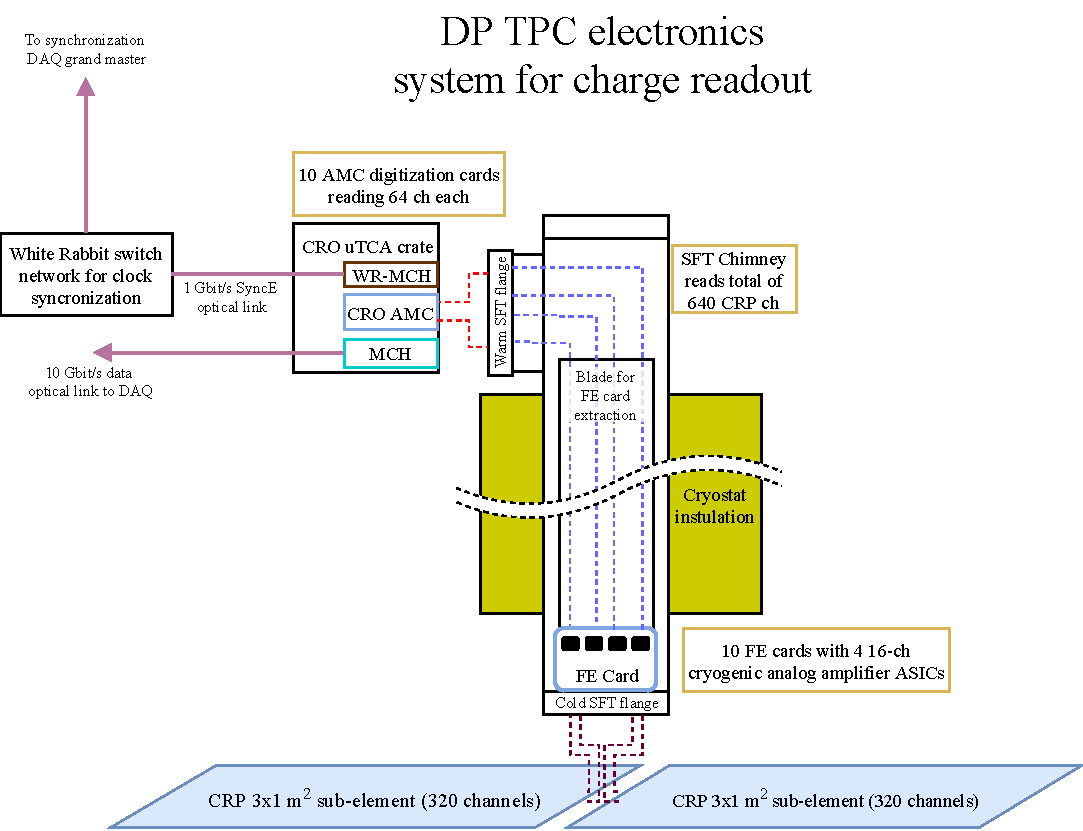
\includegraphics[width=0.6\textwidth]{dpele-crosystem-sketch}
\end{dunefigure}

The \dword{cro} electronics system, illustrated in the Figure~\ref{fig:dpele-crosystem-sketch}, is designed to provide continuous, non-zero-suppressed, and losslessly compressed digital signals by reading the charge collected on the \dwords{crp}' \SI{3}{m} long strips that are arranged in two collection views, all with a pitch of \SI{3.125}{mm}.% in the \dword{crp}. 
The system consists of %a 
the \dword{fe} analog electronics operating at cryogenic temperatures and digital electronics working in the warm environment outside of the cryostat.  The cryogenic \dshort{fe} analog electronics is based on an application-specific integrated circuit (\dword{asic}) chip with a large dynamic range (up to \SI{1200}{fC}) to cope with the charge amplification in the \dwords{crp}. The analog \dword{fe} cards are housed in dedicated \dwords{sftchimney} and are accessible from the outside even after the \dword{dpmod} is in operation, thus removing any significant risks associated with their long-term survivability. The \dwords{sftchimney} are approximately \SI{2.3}{m} long stainless steel pipes 
%\fixme{metallic cylinders?} DONE 
that traverse the entire insulation layer of the cryostat allowing placement of the \dword{fe} electronics close to the \dwords{crp} to minimize cable capacitance (noise).  In addition, their metallic structure shields the \dword{fe} cards 
from any interference from the warm digital electronics and ambient environment. The analog signals are digitized by \dwords{amc}, which are housed in the commercial \dword{utca} crates on top of the cryostat near the \dwords{sftchimney}. 

The \dword{cro} data are sampled at the rate of \SI{2.5}{MHz} with \SI{12}{bit} resolution.  
%\fixme{both cro and lro? sounds like only cro.} DONE
This frequency, traditionally used in \lartpc experiments, is well matched to the \SI{1}{\micro\second} pulse-shaping time of the \dword{fe} electronics and the detector response times determined by the electron drift velocity in the \lar. The corresponding sampling resolution along the drift coordinate is better than \SI{1}{\mm}. 

The \dword{lro} electronics system, illustrated in the Figure~\ref{fig:dpele-crosystem-sketch},  collects and digitizes the signals from the \dword{pds}, which consists of \dword{tpb}-coated \num{8}\,in \dwords{pmt} (Hamamatsu\footnote{Hamamatsu\texttrademark R5912-02-mod, \url{http://www.hamamatsu.com/}.} R5912-02-mod) located beneath the TPC cathode. The \dword{lro} electronics %should 
facilitates the detection of the primary scintillation signals, which provide the absolute time reference for the interaction events. It %should 
also enables recording the light signals generated by photons from the so-called \textit{proportional scintillation component}, the light created by the electrons extracted and amplified in the gaseous phase. A fraction of this light can reach the \dwords{pmt} after traversing the entire detector volume.  
%\fixme{what light detection element is up there?} NOW EXPLAINED  
The \dword{lro} electronics, consisting of analog and digital stages, is housed in the \dword{utca} crates on top of the cryostat structure (similar to the \dword{cro} electronics). The \dword{lro} \dword{amc} card design shares a similar architecture with the \dwords{amc} for the charge readout. The \dword{lro} \dword{utca} crates are connected to specific \dword{lro} signal \fdth flanges on top of the cryostat (see chapter~\ref{ch:fddp-pd}).
%\fixme{add: similar to the \dword{cro} electronics} is housed in the \dword{utca} crates on top of the cryostat structure.  \fixme{Need to introduce these cards before comparing them to those for the CRO}

\begin{dunefigure}[Schematic layout of the \dword{dp} \dword{lro} sub-system]{fig:dpele-lrosystem-sketch}
{Schematic layout of the \dword{dp} \dword{lro} sub-system.}
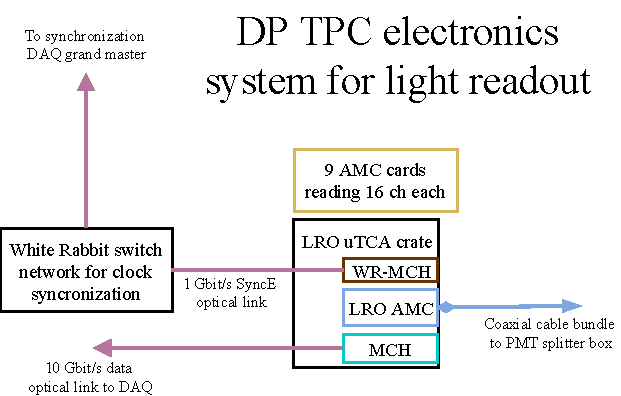
\includegraphics[width=0.6\textwidth]{dpele-lrosystem-sketch}
\end{dunefigure}

Each \dword{utca} crate for either charge or light readout is connected to the \dword{daq} system via an optical fiber link that supports at least \SI{10}{Gbit/s}. 
%\fixme{so you dont have both LRO and CRO through same chimneys to same crates; all chimneys and crates are either one or the other?} ADDED EXPLANATION
Every crate also contains a %module, 
\dword{wrmch} for the time synchronization of the digital electronics. This timing slave unit is connected via \SI{1}{Gbit/s} optical fiber to a master node that serves as a synchronization reference for all the connected slave nodes on the network. This system for the time synchronization is based on the commercially available components developed within the framework of the \dword{wr} project\footnote{\url{https://www.ohwr.org/projects/white-rabbit}.} with ad-hoc hardware and firmware development. The system performs automatic and continuous self-calibrations to account for any propagation delays and is able to provide sub-\si{\nano\s} accuracy for the timing synchronization.


%%%%%%%%%%%%%%%%%%%%%%%%%%%%%%%%%%%%%
\subsection{Design Considerations}
\label{sec:fddp-tpc-elec-des-consid}

%The principal requirements for the \dual TPC electronics system can be summarized as:
%\fixme{Could we separate out CRO and LRO? It feels like this goes back and forth. They really are separate, aren't they?  Maybe separate into CRO, LRO and common considerations...?  Also I think this section could be trimmed quite a bit.} THEY CANNOT BE SEPARATED SINCE LRO INHERITS THE SAME AMC ELECTRONICS. THE MOST NATURAL WAY IS TO INTRODUE THE CRO AND THEN LRO ELECTRONICS

The \dword{cro} electronics design covers the analog \dword{fe} cards containing pre-amplifier \dwords{asic} operating at cryogenic temperatures and digitization cards with the relevant system for their synchronization working in the warm environment outside of the cryostat. The system %should 
reads and digitizes signals from a total of \num{153600} channels (per one \dword{dpmod}) and is capable of continuously streaming the collected and losslessly compressed data to the \dword{daq} without any zero suppression. 
The design of the \dshort{cro} electronics system was developed to fit the following requirements:
\begin{itemize}
\item{The \dword{cro} electronics %must be able to 
shall measure signals of up to \SI{1200}{\femto\coulomb} without saturation; this has been optimized following \dword{mc} studies on the maximal occupancy per channel in shower events~\cite{WA105_TDR}. For a nominal \dword{crp} gain of \num{20}, a \dword{mip} signal is expected to be around \SI{30}{fC} -- the lowest limit that assumes a particle travelling horizontally with an azimuthal angle of \num{0} degrees -- giving %the 
a maximal operational range of up to \num{40} \dwords{mip}.}

\item{The electronic noise in the \dshort{cro} analog electronics is required to be \SI{< 2500}{e^{-}}. This condition can be derived from the requirement on the minimal \dword{s/n}, which should be greater than \num{5}:\num{1} once the charge attenuation is taken into account. Given the maximum drift distance of \SI{12}{\meter}, the largest attenuation factor due to electro-negative impurities assuming the \SI{3}{\milli\second} (minimally required) electron lifetime and the drift field of \SI{0.5}{\kilo\volt/\cm} is \num{0.08}. The smallest \dword{mip} signal with the \dword{crp} effective gain of \num{20} is therefore \SI{2.5}{\femto\coulomb} (\SI{15600}{e^{-}}).}

\item{The peaking time of the \dword{fe} analog amplifiers %should 
shall be \SI{1}{\micro\second}. This requirement is driven by the need for optimal vertex resolution, determined in turn by the single track resolution and the power to separate two or more tracks that are close to one another.}

\item{The sampling frequency %should 
shall be \SI{2.5}{\MHz} to match the peaking time of the \dword{fe} electronics.}

\item{The power dissipated by the \dword{fe} analog electronics %must 
shall be below \SI{50}{\milli\watt/channel} in order to minimize the heat input to the cryostat volume.}

\item{The \dword{fe} analog electronics %should 
shall be replaceable without the risk of contaminating the main \lar volume in order to guarantee the long-term reliability of the system.}

\item{The \dword{adc} resolution %should 
shall be such that the noise is at the level of an \dword{adc}
%\fixme{does not exceed?} the level of an \dword{adc}, %while THIS WAS CORRECT
given a dynamic range wide enough to match the response of the \dword{fe} amplifier. This can be achieved with a \num{12} bit \dword{adc}.}

\item{The digital electronics to be placed outside of the cryostat in the warm environment %can 
shall be capable of adopting standard industrial components and solutions, to keep the costs lower and to benefit from  %ensuring low costs and benefiting of the 
technological evolution, e.g., higher network speeds.}
\end{itemize}
As described %in the details 
in subsequent sections, the achieved performance of the final system is significantly better with respect to many of the listed requirements.  %\fixme{above sentence not clear: performance exceeds requirements? (anne)} YES, THERE WERE MINIMAL REQUIREMNTS COMING FROM EXPERIENCE WITH SP DETECTORS

The magnitude of the noise also %plays a role in 
has an effect on the quality of the lossless compression of the raw data. % performed by the digital electronics. 
A compression factor of about \num{10} is achieved with the \rms noise level below \SI{1}{\dword{adc}}. To give an idea of the compression efficiency dependency on the noise level a compression factor of four is obtained with the noise at around \SI{1.5}{\dword{adc}} counts. 
%\fixme{What are you saying here: ``we're expecting 1.5 ADC so we'll only get factor of 4, but wouldn't it be nice to get factor of 10''? If that's your meaning, what's keeping you from getting the noise low enough?} REFORMULATED THE SENTENCE
% A compression factor of \num{7} can be achieved with a \rms noise level of $\sim$ \SI{1.5}{\dword{adc}}, increasing to \num{10} for \rms noise levels below \SI{1}{\dword{adc}} \rms.

%Given the amplification of the ionization charge in \dword{crp}, the electronics needs to be sensitive to the signals over a large dynamic range (up-to \num{40} times the \dword{mip}-level signals for a nominal \dword{crp} gain of %\num{20} or \SI{1200}{\femto\coulomb}) to avoid saturation of the analog inputs by large localized energy disposition produced, for example, in shower events. The minimal requirelemt on the intrinsic noise %of the \dword{fe} analog electronics is \SI{<2500}{e^{-}}.  The condition is derived from the requirement on the minimal \dword{s/n} of \num{5:1} as in the SP design. Given the maximal drift \SI{12}{\meter} the %largest attenuation factor due to electro-negative impurities assuming the nominal \SI{3}{\milli\second} electron lifetime is \num{0.08}. The smallest \dword{mip} signal with the \dword{crp} effective gain is therefore %\SI{2.5}{\femto\coulomb} (\SI{15600}{e^{-}}).

%The charge amplification provided by the \dword{crp} loosens requirements on the intrinsic noise of the \dword{fe} analog electronics. For the \dword{crp} nominal gain of \num{20}, the signal-to-noise ratio for a \dword{mip} signal %(\SI{30}{fC}) should be around \num{100}, which would not pose any problems for the detection/reconstruction. 

The primary objective of the \dword{lro} system is to detect signals, from a minimum of one \phel on one \dword{pmt}, giving a precise timestamp that can be used in conjunction with the charge signals to determine the absolute event time ($T_0$). 
%\fixme{why insert (drift)?} MODIFIED
Precise measurements of \dword{lro} signal charge allow the continual monitoring of the \dword{pmt} gain at the single \phel level, and the determination of the number of photons in each scintillation event.  In addition, an \dword{adc}  continuously streams data, downsampled to \SI{400}{ns} as for the \dword{cro} signals,  which, amongst other items, allows measurements of the scintillation time profile. In addition, the \dword{lro} system reads \num{20} channels from reference SiPM sensors from the \dword{pd} calibration system.
%\fixme{``...number of signals from the \dword{pd} calibration trigger and about \num{20} channels from calibration reference sensors.'' (?)} EXAPLAINED BETTER 

The cryogenic analog electronics for the \dword{cro} is housed in the dedicated \dwords{sftchimney}. %Their 
Its design %must 
enables access to the \dword{fe} card for possible replacement without %any 
risk of contaminating the pure \lar in the main cryostat volume. The chimneys %must 
possess a cooling system that can control the temperature around the \dword{fe} cards to roughly \SI{110}{\kelvin} %for their optimal noise. 
to reach their optimal noise level and %. In addition, the cooling system must 
that compensates for the heat input from the chimneys into the cryostat volume. 

The digital electronics for both charge and light readout is located in the warm environment on the top of the cryostat supporting structure and is therefore easily accessible. This fact removes any constraints associated with the accessibility and operation in cryogenic environments allowing for the usage of standard components and industrial solutions in the design. Digital electronics must be continuously and automatically synchronized to better than \SI{400}{\nano\s} to ensure the correct temporal alignment of the \dword{adc} samples from all of the readout channels. This is a minimal requirement dictated by the fact that the sampling rate is \SI{2.5}{\MHz}.  

%Some of the k
Key parameters for the electronics system design are summarized in Table~\ref{tab:dpele-physicsparams}. %The requirements for the \dual electronics system are documented in DUNE-docdb-6428.

\begin{dunetable}
[Parameters for the TPC electronics system design]
{lr}
{tab:dpele-physicsparams}
{Parameters for the  TPC electronics system design. The numbers are given for one \dword{dpmod}.}   
Parameter & Value  \\ \toprowrule
  \dword{cro} channels    &  \num{153600}            \\ \colhline
  \dword{cro} continuous sampling rate & \SI{2.5}{\MHz}\\ \colhline
  \dword{cro} \dword{adc} resolution & \num{12}\,bit           \\ \colhline
  \dword{cro} data compression factor   & \num{10}    \\ \colhline 
  \dword{cro} data flow  & \num{430}\,Gibit/s          \\ \colhline 
  \dword{lro} channels       & \num{720}               \\ \colhline
  \dword{lro} continuous sampling rate & \SI{2.5}{\MHz} \\ \colhline
  \dword{lro} \dword{adc} resolution & \num{14}\,bit            \\ \colhline
  \dword{lro} data compression factor  & \num{1}       \\ \colhline
  \dword{lro} data flow   & \num{24}\,Gibit/s          \\ 
\end{dunetable}
%\fixme{Gibit instead of Gbit?} YES, SINCE THEN NUMBERS WERE COMPUTED IN THE BASE OF 1024, CHECKED WITH BRETT


%%%%%%%%%%%%%%%%%%%%%%%%%%%%%%%%
\subsection{Scope}
\label{sec:fddp-tpc-elec-scope}

The scope of the TPC electronics system covers the procurement, production, testing, validation, installation, and commissioning of all the components necessary to ensure the complete readout of the charge and light signals from a given \dword{dpmod}. This includes: %The covered items are the following:
\begin{itemize}
\item{Cryogenic analog \dword{fe} cards for charge readout;}
\item{\dword{amc} cards for charge and light readout;}
\item{The \dword{wrmch} cards for \dword{amc} clock synchronization;}
\item{\dword{utca} crates;}
\item{Switches for the \dword{wr} network;}
\item{\dwords{sftchimney};}
\item{Low-voltage power supplies, distribution, and filtering system for the \dword{fe} cards;}
\item{Flat cables connecting the \dword{fe} cards to the warm flange interface of the \dwords{sftchimney};}
\item{VHDCI cables connecting the warm flange interface of the \dwords{sftchimney} to \dwords{amc}.}
\end{itemize}

%\fixme{what about cables/connections to the \dwords{crp} and \dwords{pmt}?} THEY ARE PROVIDED BY OTHER CONSORTIA AS COVERED IN THE INTERFACE SECTION

The total numbers for components to be procured to instrument one \dword{dpmod} are given in Table~\ref{tab:dpele-num-components}

\begin{dunetable}
[Numbers for \dual electronics components to procure]
{lr} {tab:dpele-num-components}
{Numbers for \dual electronics components to procure for one \dword{dpmod}.}
Name & Number  \\ \toprowrule
\dword{cro} cryogenic \dwords{asic} (\num{16} ch) & \num{9600} \\ \colhline
\dword{cro} cryogenic analog \dword{fe} cards (\num{64} ch) & \num{2400} \\ \colhline
\dword{cro} \dwords{amc} & \num{2400} \\ \colhline
\dwords{sftchimney} & \num{240} \\ \colhline
Flat cables for \dword{sftchimney} (\num{68} ch) & \num{2400} \\ \colhline
Flat cables for \dword{sftchimney} (\num{80} ch) & \num{2400} \\ \colhline
VHDCI cables (\num{32} ch) & \num{4800} \\ \colhline
\dword{lro} \dwords{amc} with analog \dword{fe} & \num{45} \\ \colhline
\dword{utca} crates & \num{245} \\ \colhline
\dword{wrmch} units & \num{245} \\ \colhline
WR switches (\num{18} ports) & \num{16} \\ 
\end{dunetable}


%%%%%%%%%%%%%%%%%%%%%%%%%%%%%%%%%%%%%%%%%%%%%%%%%%%%%%%%%%%%%%%%%%%%
\section{TPC Electronics System Design}
\label{sec:fddp-tpc-elec-design}

%\fixme{separate CRO and LRO} THERE IS STRONG COUPLING BECAUSE THE LRO INHERITS THE DESIGN FROM CRO. IT IS NOT EVIDENT HOW TO DO THIS IN CLEAR CUT WAY

The \dword{cro} \dword{fe} analog electronics is based on a cryogenic \dword{asic} chip with a large dynamic range (up to \SI{1200}{\femto\coulomb}) to accomodate the charge amplification in the %\dual 
\dword{crp}. The \dword{fe} cards read \num{64} \dword{crp} channels each. They are mounted in dedicated  \dwords{sftchimney} and are located within a short distance (\SI{<1}{\metre}) from each \dword{crp} to minimize the noise caused by long cables (large cable capacitance). The cards remain accessible throughout the \dword{dpmod} operation. Each \dword{sftchimney} %hosts 
accommodates \num{10} \dword{fe} analog cards, which corresponds to the readout of \num{640} \dword{crp} channels per chimney. There are, therefore, \num{240} \dwords{sftchimney} to be installed for the charge readout in a given \dword{dpmod}.   

The differential analog signals from the analog \dword{fe} cards, carried by the twisted-pair ribbon cables and routed via an interface flange of the \dwords{sftchimney}, are digitized by the \dword{amc} cards located %in the warm conditions 
outside of the cryostat. These cards are %hosted 
installed in \dword{utca} crates placed in the immediate vicinity of the \dwords{sftchimney} (one crate per chimney). %In the baseline version of the design currently used for \dword{pddp}, each \dword{amc} digitizes \num{64} channels corresponding to reading one \dword{fe} analog card. Each \dword{utca} in such case contains \num{10} \dwords{amc} reading a total of \num{640} channels. However, an implementation with \dwords{amc} supporting a higher channel density is also being investigated for cost reduction purposes.
In the design for \dword{pddp}, each \dword{amc} digitizes \num{64} channels, corresponding to reading one \dword{fe} analog card. Each \dword{utca}  contains \num{10} \dwords{amc} reading a total of \num{640} channels. However, an implementation with \dwords{amc} supporting a higher channel density is being investigated for cost-reduction purposes. 
%\fixme{I need a picture showing the AMC, the \dword{fc} card, and the \dword{utca}!} ALL THESE PICTURES ARE PROVIDED LATTER WHEN THE RESPECTIVE UNIT IS DESCRIBED

The \dword{lro} \dword{fe} analog and digital electronics is based on a custom-built \dword{amc}. The card contains a \dword{catiroc} \dword{asic} \cite{Blin:2017}, which is used to determine %precisely 
the charge and start times of signals from each individual \dword{pmt} to high precision. In addition, a \SI{14}{bit} \SI{65}{MHz} \dword{adc} digitizes the data for continuous streaming of the \dword{pmt} signals. Each card reads up to \num{16} channels. A potential %future 
upgrade is to increase the channel density per card to \num{32} channels. The \dword{lro} cards are housed in five dedicated \dword{utca} crates located close to the \dword{pmt} instrumentation \fdth{}s.

\begin{dunefigure}[Top corner view of \dword{dpmod}]{fig:dpele-sft-chimney-pattern}
{Corner view of \dword{dpmod} showing the pattern of the \dwords{sftchimney} and \dword{utca} crates for charge readout above \dwords{crp}.}
\includegraphics[width=0.6\textwidth]{dpele-sft-chimney-pattern}
\end{dunefigure}
%\fixme{Need a similar picture for the LRO system. anne} SAME AS ABOVE

Every \dword{utca} crate contains a network switch, \dword{mch}, via which the data are sent to the  \dword{daq} and to %as well as a module 
a (\dword{wrmch}) for %clock/ 
time synchronization and trigger timestamp distribution to the \dwords{amc}. Both \dword{mch} and \dword{wrmch} require one optical fiber link each. 

The \dword{mch} switch streams the data from \dwords{amc} via a dedicated optical link. Currently \dword{pddp} uses \dword{mch} operating at \SI{10}{Gbit/s}. However, a move to \SI{40}{Gbit/s} links for the \dword{dpmod} implementation is under consideration because of the technology evolution with associated cost reductions and a possible increase in the channel density of each \dword{amc}.

The \dword{wrmch} time synchronization unit is based on the \dword{wr} system, which provides hardware and protocols for the network-based sub-\si{\nano\s} synchronization between a master and different slave nodes. The connection of the \dword{wrmch} to the \dword{wr} network is done via \SI{1}{Gbit/s} synchronous Ethernet optical link. \dword{wrmch} distributes the timing information for synchronization of the \dwords{amc} via the \dword{utca} backplane. In addition, this unit can be used to transmit triggers to the digitization units within the crate. This is achieved by sending it dedicated data packets containing trigger timestamp information. 

Figure~\ref{fig:dpele-sft-chimney-pattern} shows a corner view of the \dword{dpmod} illustrating the pattern of the \dwords{sftchimney} and the attached \dword{utca} crates above the \dwords{crp}. Each crate/\dword{sftchimney} collects signals from \SI{3}{\meter} long strips of two \SI[product-units=power]{1x3}{\meter} \dword{crp} segments. Each chimney completely %traverses 
penetrates the cryostat insulation layers (not shown in the figure). 
%A cut-out view of the chimney illustrates the location of the \dword{fe} cards and provides the overall scale of this object. 


\begin{dunetable}
[Summary of some of the principal %numbers 
parameters of the TPC electronics system.]
{lr} {tab:dpele-numparts}
{Summary of some of the principal %numbers 
parameters  of the TPC electronics system for charge and light readout of a \dword{dpmod}.}
Name & Number  \\ \toprowrule
   \dword{cro} \dwords{sftchimney}/\dword{utca} crates              &  \num{240}   \\ \colhline
   \dword{cro} channels per \dword{sftchimney}/\dword{utca} crate & \num{640} \\ \colhline
   \dword{cro} cryogenic analog \dword{fe} cards per \dword{sftchimney}    &  \num{10}     \\ \colhline
%   \dword{cro} Cryogenic analog \dword{fe} cards (total)                   & \num{2400}  \\ \colhline
   \dword{cro} \dwords{amc} per \dword{utca} crate                       & \num{10}      \\ \colhline
%   Charge readout \dwords{amc} (total)                                   & \num{2400}      \\ \colhline 
   \dword{lro} \dword{fe} cards  per \dword{utca} crate & \num{9} \\ \colhline
%   Light readout \dword{fe} cards (total)           & \num{45} \\ \colhline
   \dword{lro} channels per \dword{utca} crate & \num{144} \\ \colhline
   \dword{lro} \dword{utca} crate                      & \num{5} \\ \colhline
   \dword{wrmch} per \dword{utca} crate                 & \num{1} \\ 
%   \dword{wrmch} (total)                              & \num{245} \\ \colhline
%   \dword{utca} crates (total)                         & \num{245} \\ \colhline
\end{dunetable}

A short summary of some of  the number of principal components and channel granularity in the design of the \dual electronics is provided in Table~\ref{tab:dpele-numparts}. 

%%%%%%%%%%%%%%%%%%%%%%%%%%%%%%%%%%%
\subsection{Cryogenic Analog Front-end Electronics}
\label{sec:fddp-tpc-elec-design-cryofe}

The cryogenic amplifier \dword{asic} is the main component of the \dword{fe} analog cards. Its design is based on the CMOS \SI{0.35}{\micro\meter} technology and is an outcome of an R\&D  activity started in 2006, which resulted in several versions of the cryogenic amplifier for both \single and \dual \dword{lartpc} detectors. Two principal versions of \dword{asic} chips have been produced for \dual \dword{lartpc} operation. In the first version the amplifiers have a constant gain in signal inputs of \numrange{0}{1200}\,\si{\femto\coulomb} (\numrange{0}{40} \dword{mip}). In the second, the amplifiers have a higher linear gain for signals up to \SI{400}{\femto\coulomb} (roughly \num{10} \dword{mip} signals) and a logarithmic response in the \numrange{400}{1200}\,\si{\femto\coulomb} range. This double-slope behavior is obtained by using a MOSCAP capacitor in the feedback loop of the amplifier that changes its capacitance above a certain signal threshold. The aim of this solution is to optimize the resolution for few-\dword{mip} charge depositions while preserving the overall large dynamic range of the amplifier.

\begin{dunefigure}[Cryogenic \dword{fe} \dword{asic} properties]{fig:dpele-fe-asic-prop}
{Cryogenic \dword{fe} \dword{asic} properties: amplifier response (left) and noise (right) at different temperatures measured at the output of differential buffer.}
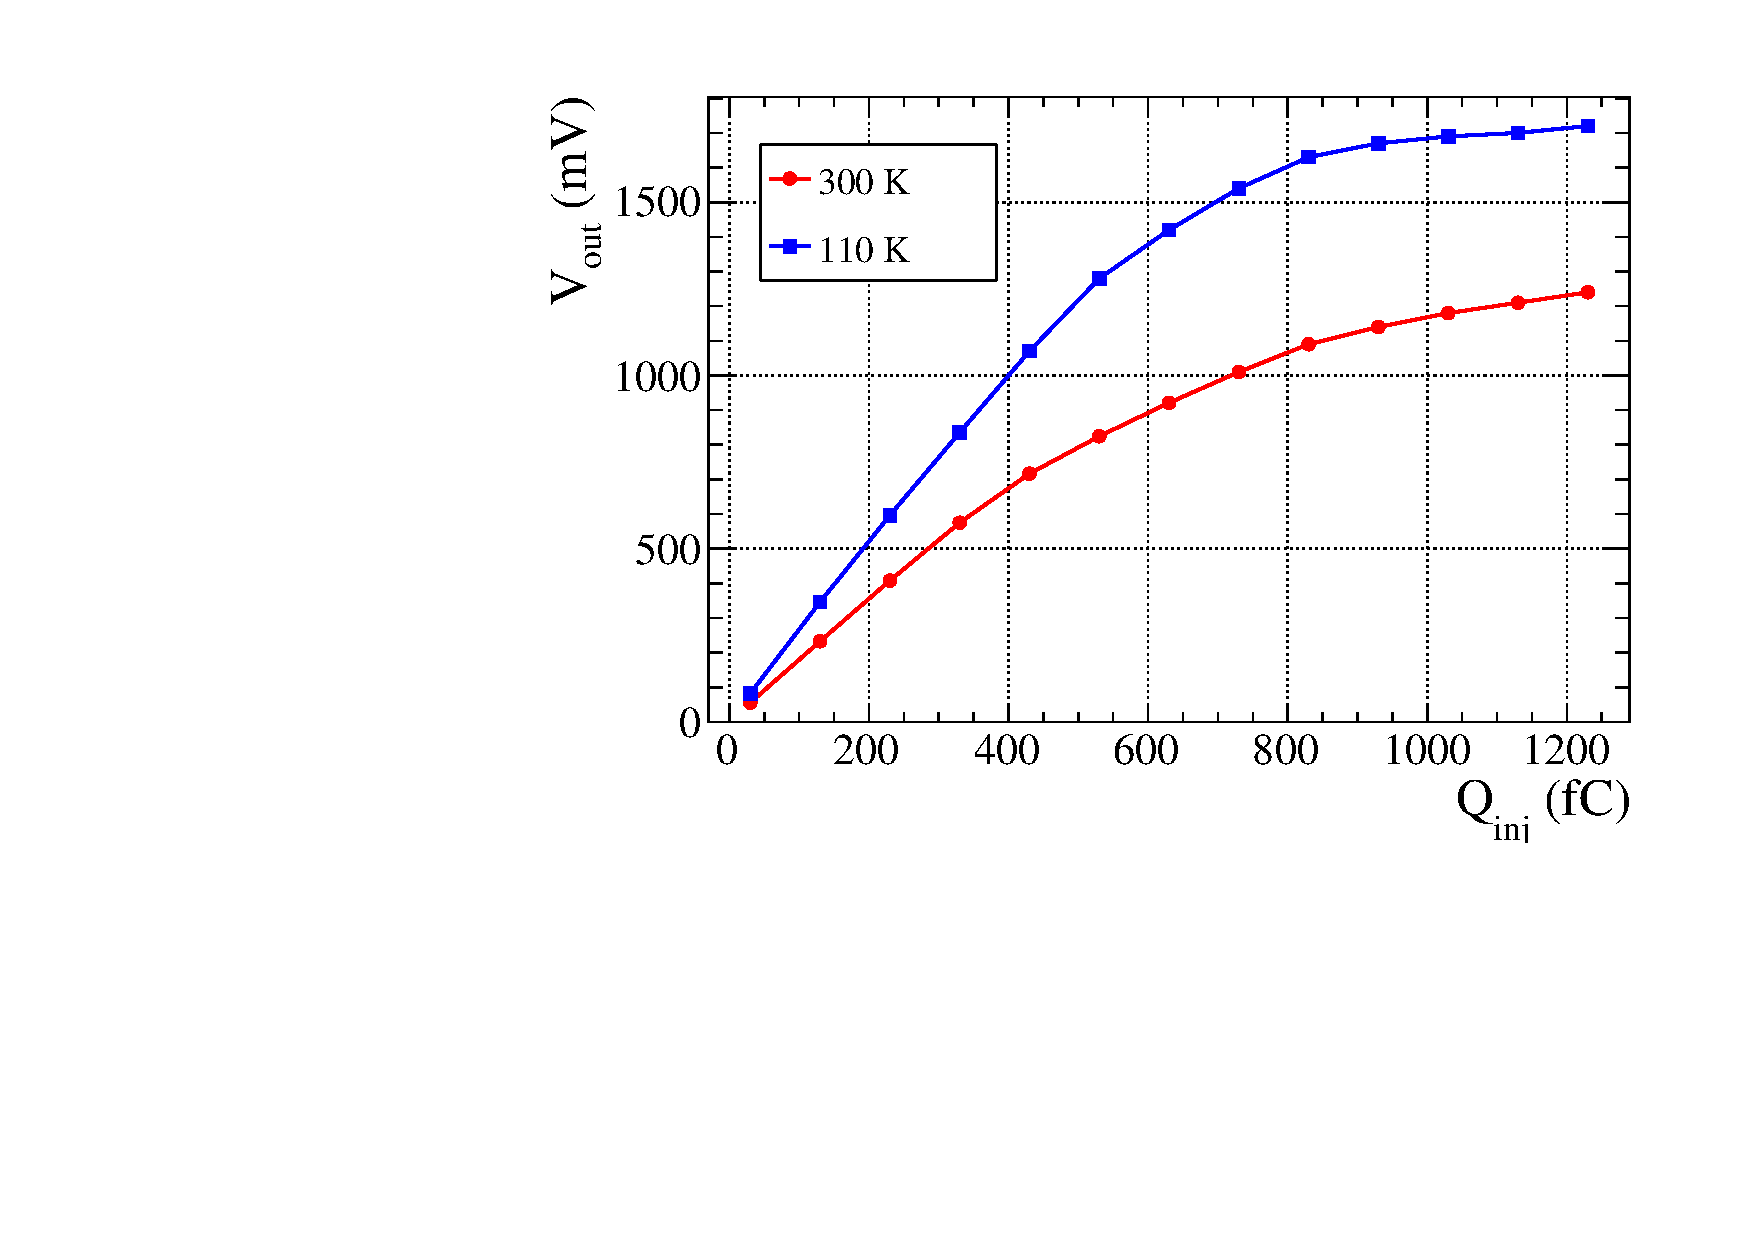
\includegraphics[width=0.49\textwidth]{dpele-fe-asic-gain}
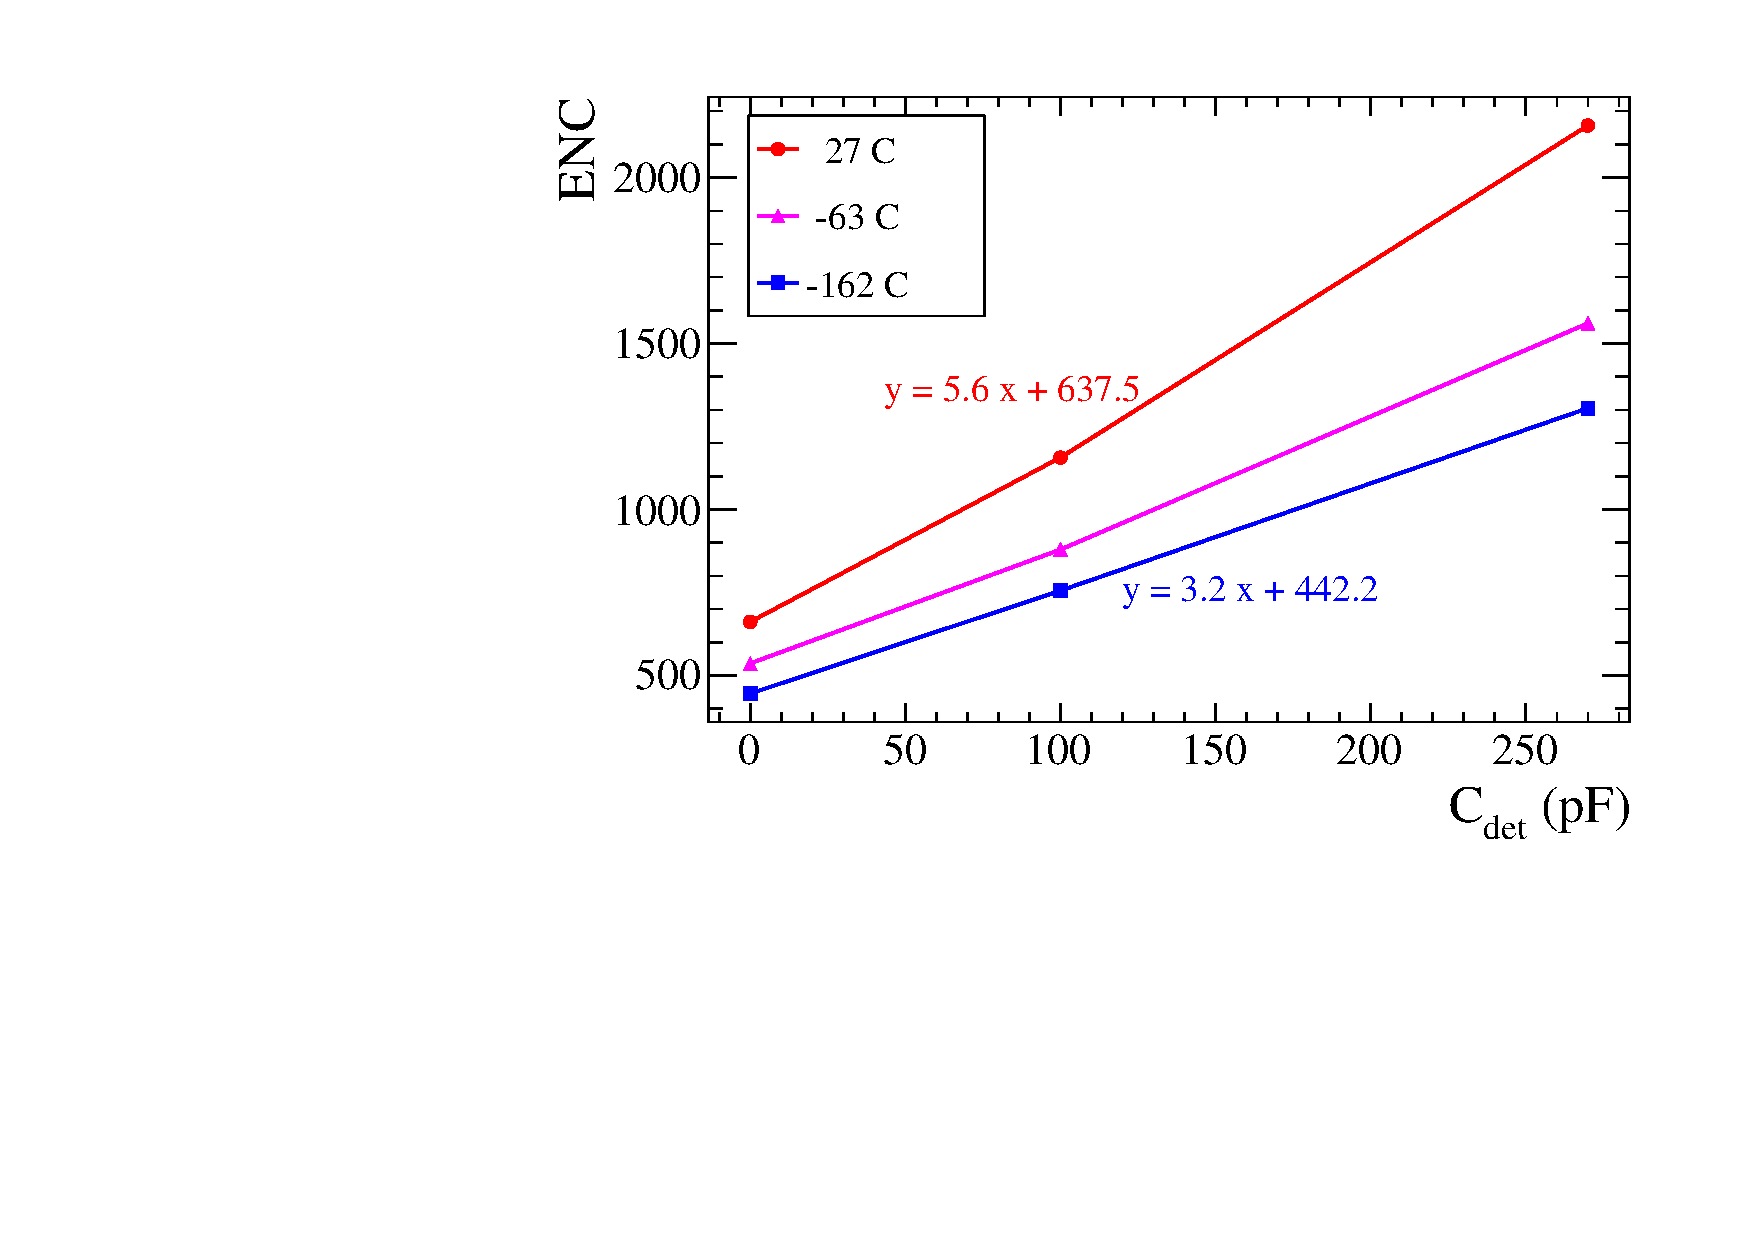
\includegraphics[width=0.49\textwidth]{dpele-fe-asic-noise}
\end{dunefigure}

%Figure~\ref{fig:dpele-fe-asic-noise} 
The \dword{asic} version with the double-slope gain was selected for \dword{pddp} and has been adopted for the \dual TPC electronics design. The left plot in Figure~\ref{fig:dpele-fe-asic-prop} illustrates the response of this amplifier for different values of the injected charge, while that on the right shows the measured noise in units of Equivalent Noise Charge (ENC) as a function of the detector capacitance at different temperatures. 
%\fixme{why in quotes?} REMOVED
For the \dword{crp} anode (detector) capacitance of \SI{480}{\pico\farad} per \SI{3}{\metre} strip, the expected noise is around \SI{2000}{e^{-}} at \SI{110}{\kelvin}. Each \dword{asic} contains \num{16} amplifier channels with differential line buffers and has a power consumption of \SI{11}{\milli\watt/channel}, surpassing the \SI{< 50}{\milli\watt/channel} requirement. 

\begin{dunefigure}[Image of an analog \dword{fe} card mounted on the extraction blade]{fig:dpele-fe-card-blade-image}
{Image of an analog cryogenic \dword{fe} card mounted on the extraction blade, which is a part of the \dword{sftchimney} sub-system.}
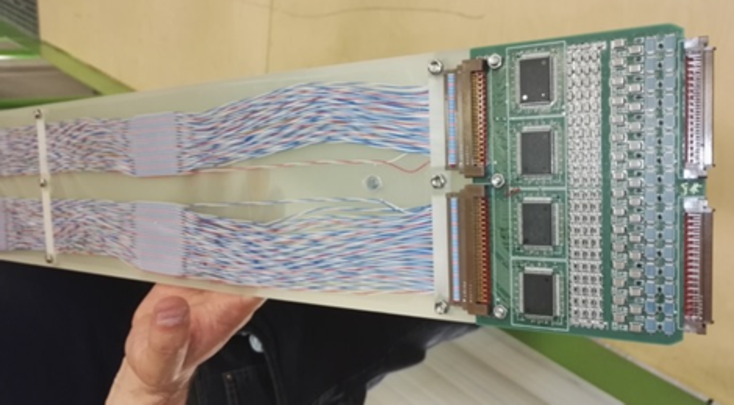
\includegraphics[width=0.7\textwidth]{dpele-fe-card-blade-image}
\end{dunefigure}
%\fixme{extraction blade is defined lower down; to fix} ADDED AN EXPLANATION THAT IT IS PART OF THE SFT CHIMNEY. IT IS ALSO COVERED IN THE GENERAL OVERVIEW SECTION

Each cryogenic \dword{fe} card, shown in Figure~\ref{fig:dpele-fe-card-blade-image}, %hosts 
holds four \dword{asic} amplifier chips and a few passive discrete components. The input stage of each amplifier channel has a \SI{1}{\giga\ohm} resistor to ground followed by a \SI{2.2}{\nano\farad} decoupling capacitor; both are rated for \dword{hv} operation. The %function of the 
resistor grounds the \dword{crp} anode strips. A TVS diode\footnote{Bourns\texttrademark{} CDSOD323-T08LC TVS diode.} protects each input stage against discharges coming from the \dword{dpmod}. This component was selected after studying the performance of different devices for the electrostatic discharge protection by subjecting them systematically to discharges of a few \si{kV} with an energy similar to that of the \dwords{lem} in the \dword{crp}. The \dword{fe} cards also house the blocking capacitors for further filtering of the low-voltage power lines. These are first filtered at the power supply and transported via shielded cables.

\begin{dunefigure}[Noise measurements in the \dword{wa105} in different conditions]{fig:dpele-311-noise}
{Noise of measurements in the \dword{wa105} in different conditions. Left: warm with the slow control cables connected to the cryostat flanges (red points) and disconnected (black points). Right: warm (red points) and cold (black points) with the slow control cables disconnected. The channels with negative (positive) channel number correspond to the strips of \SI{3}{\meter} (\SI{1}{\meter}).}
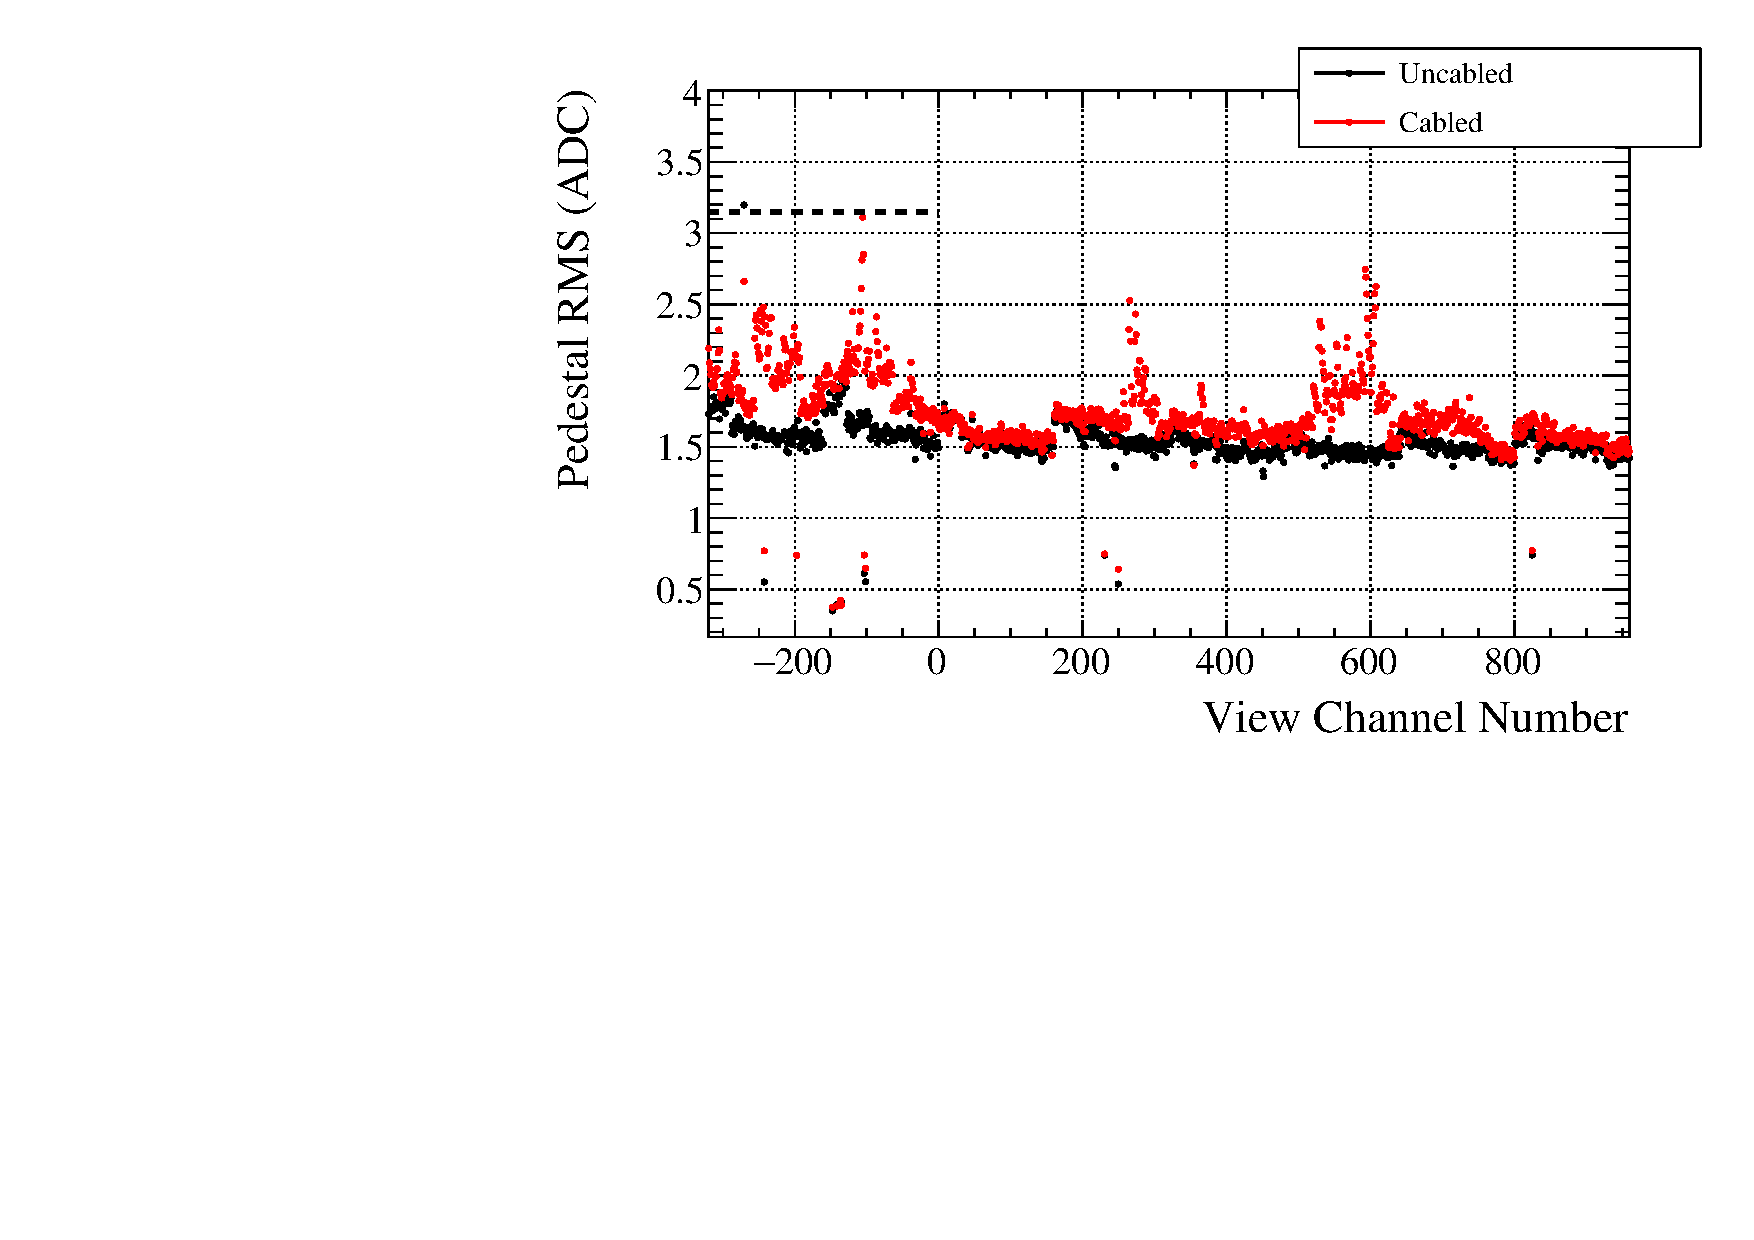
\includegraphics[width=0.45\textwidth]{dpele-311-noise-warm}
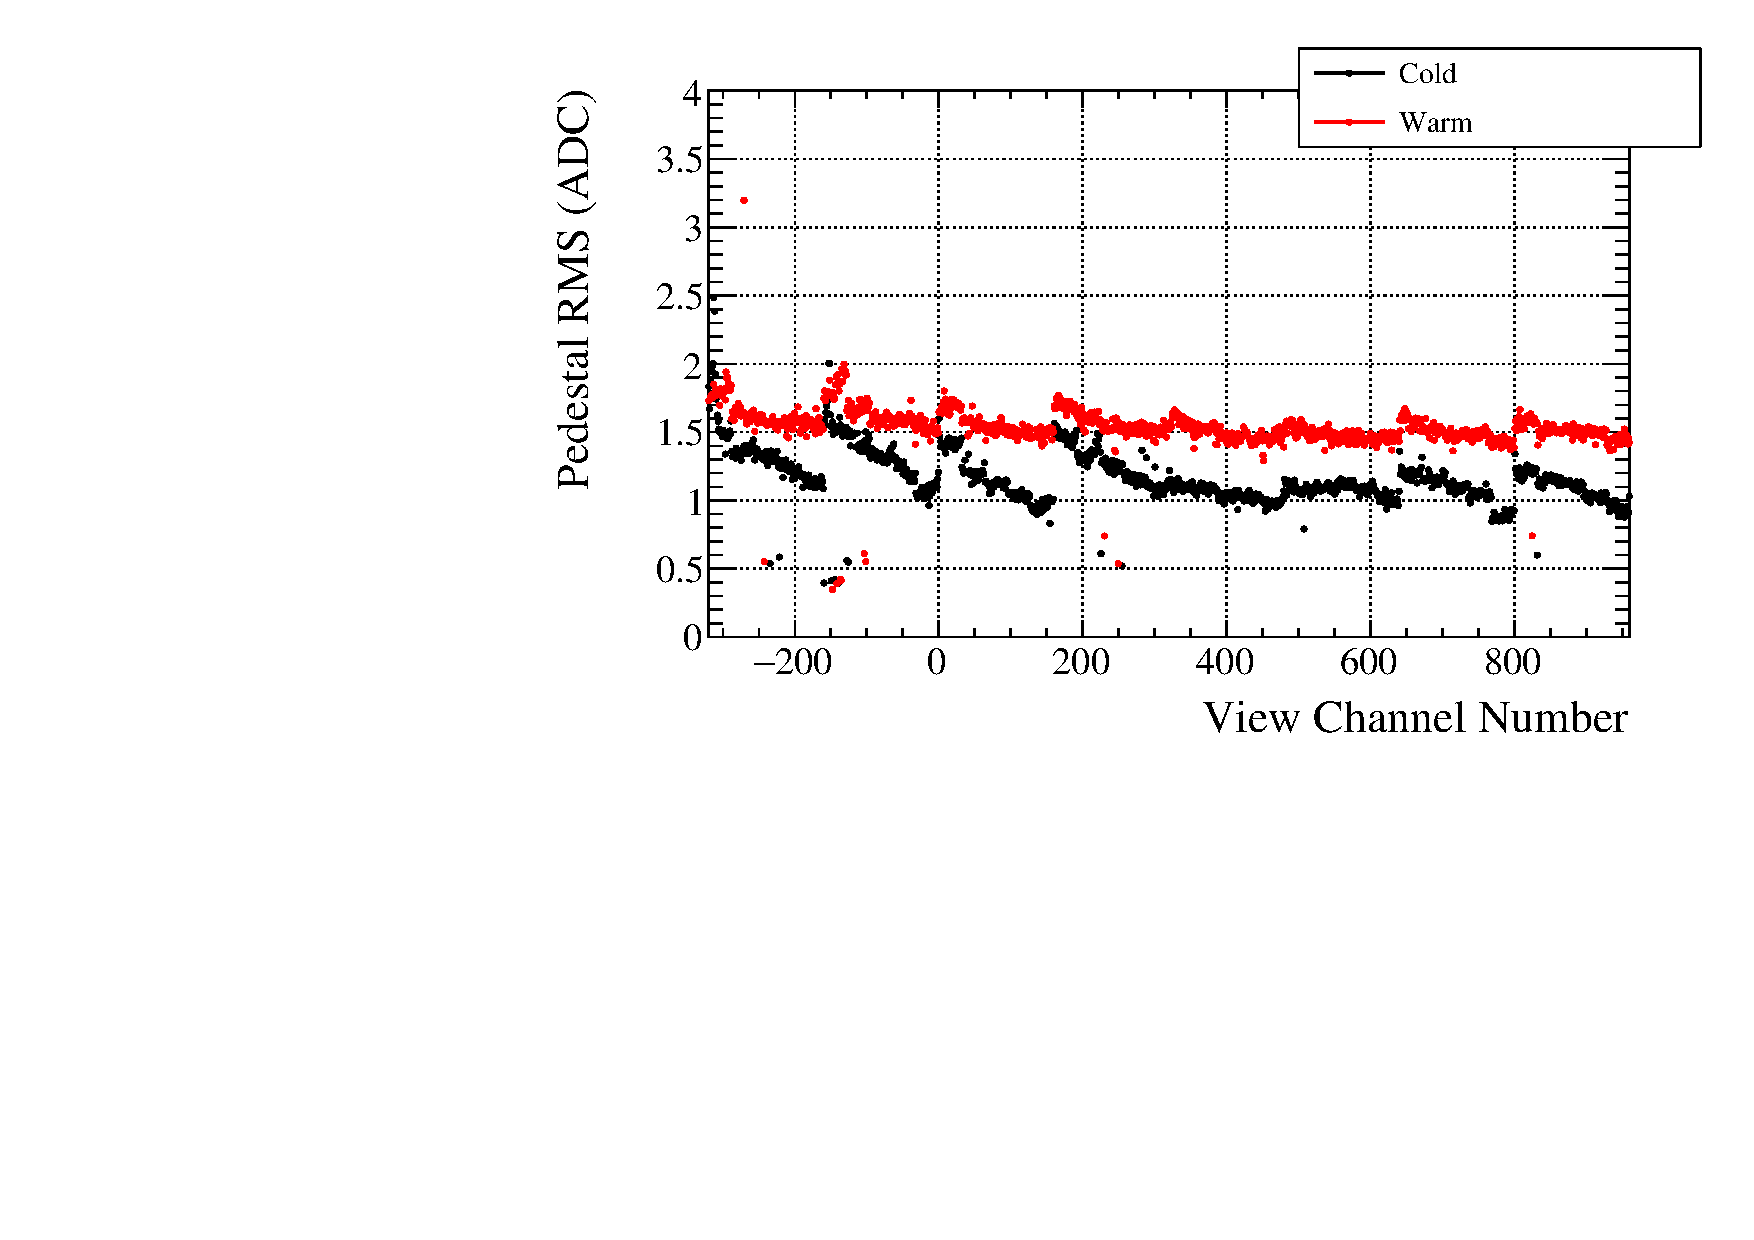
\includegraphics[width=0.45\textwidth]{dpele-311-noise-warm-cold}
\end{dunefigure}

%While 
Although the \dword{fe} amplifier \dwords{asic} are in a shielded environment provided by the chimneys, which act as Faraday cages,
%\fixme{``which act as'' Faraday cages?} DONE 
interference from other equipment (via a noisy ground or ground loops) could significantly worsen the noise performance from the design target. Figure~\ref{fig:dpele-311-noise} shows %some 
results of %the 
noise measurements performed under different conditions in the \dword{wa105}. The channels reading \SI{3}{\meter} (\SI{1}{\metre}) long strips correspond to negative (positive) channel numbering in the plots and the \num{1} \dword{adc} count is equivalent to about \num{900} electrons. The left plot of Figure~\ref{fig:dpele-311-noise} shows the noise measurements performed at warm temperature with and without slow control cables (\dword{crp} \dword{hv}, \dword{crp} motors, level meters, temperature probes, etc.) connected. 
%\fixme{stuff in parentheses all pertain to slow controls?} YES THESE LIST EXAMPLES OF THE E\dword{lem}ENTS OF THE 311 SLOW CONTROL SYSTEM WHICH WERE NOT GROUNDED IN A CLEAN WAY
The noise is clearly affected by the grounding of the slow controls: the average value of the noise \rms is around \num{1.7} \dword{adc} with slow control cables connected, and decreases to about \num{1.5} \dword{adc} counts when they are removed. %As explained later,
%\fixme{ref section} IT IS EXPLAINED AT THE END OF THIS SECTION
The grounding scheme of the \dword{wa105} does not correspond to the one %foreseen for DUNE, 
planned for the \dword{dpmod}, where all electrical equipment is referred uniquely to the cryostat ground and is completely insulated from the external environment. 

One interesting feature, particularly visible with the cables disconnected, is %that the noise measured in \dword{wa105} is similar for the channels connected to the \SI{1}{\meter} and \SI{3}{\meter} long strips. 
the similarity of the noise measured for the channels connected to the \SI{1}{\meter} and \SI{3}{\meter} long strips in the \dword{wa105}. 
Given that the longer strips have %thrice 
three times the input capacitance of the shorter ones, the expected noise (see Figure~\ref{fig:dpele-fe-asic-prop}) for these should be larger by about a factor of two as indicated by the dashed line in the plot. In addition, the noise on the short strips is lower than expected (\num{1.5} \dword{adc}) for the \SI{160}{pF/m} strip input capacitance (\num{1.7} \dword{adc}). The reason for this behavior %of the noise in the \dword{crp} of 
in the \dword{wa105} is still under investigation. %However, 
Measurements have already shown that the capacitance of the \dword{crp} anode strips is not purely to ground, but rather it is driven by the inter-strip couplings, which creates a more complicated electrical network. 

Figure~\ref{fig:dpele-311-noise} (right) also shows a comparison of the noise measurements in the \dword{wa105} taken with the \dword{fe} electronics at warm (red points) and cold (black points) at around \SI{150}{\kelvin}. The slow control cables were disconnected in both cases. However, the cold measurements were performed with the recirculation pump active and the cathode \dword{hv} connected. 
%\fixme{present? means hv was connected?} DONE
The \rms noise averaged over all channels decreases by about 25\% from roughly \SI{1.5}{\dword{adc}} to \SI{1.1}{\dword{adc}} when the \dword{fe} analog cards are cold. For comparison, the expected signal for a \dword{mip} with the \dword{crp} gain of \num{20} should be around \SI{200}{\dword{adc}} counts. %\fixme{counts?} DONE

The overall grounding principle of the \dword{wa105} was based on %having 
using the cryostat as the ground reference. The low-voltage power supplies for the \dword{fe} analog electronics and the \dword{utca} crates were powered %via 
using insulating transformers to ensure that %they could see 
no other ground could interfere. %On the other hand, 
In contrast, the design of the slow control system did not include any insulation transformers. This equipment was grounded to the building electrical network, thereby creating an interference with the ground of the cryostat. Stricter treatment of the ground connections, as %foreseen 
implemented for \dword{pddp} and planned for the \dword{dpmod}, and a lower \dword{sftchimney} operating temperature of around \SI{110}{\kelvin} (from \SI{150}{\kelvin}) should help to further reduce the noise %levels 
from the levels observed in the \dword{wa105}.


%%%%%%%%%%%%%%%%%%%%%%%%%%%%%%%%%%%
\subsection{Signal Feedthrough Chimneys}
\label{sec:fddp-tpc-elec-design-sft}

The \dwords{sftchimney} are designed to enable access to the \dword{fe} analog electronics for a potential repair or exchange while the \dword{dpmod} is filled and in operation. % (filled with the \lar). 
In addition, their metallic structure acts as a Faraday cage isolating the \dword{fe} \dwords{asic} from environmental interference.  Each \dword{sftchimney} hosts \num{10} analog cryogenic \dword{fe} cards (reading \num{640} channels in total).  %Some of the 
Details of the design are illustrated in Figure~\ref{fig:dpele-sft-chimney-design}. 
%\fixme{diff between ``SFT chimney'' and just SFT?} FIXED, WAS MISSING CHIMNEY

\begin{dunefigure}[Details of the \dword{sftchimney} design]{fig:dpele-sft-chimney-design}
{Details of the \dword{sft} chimney design.}
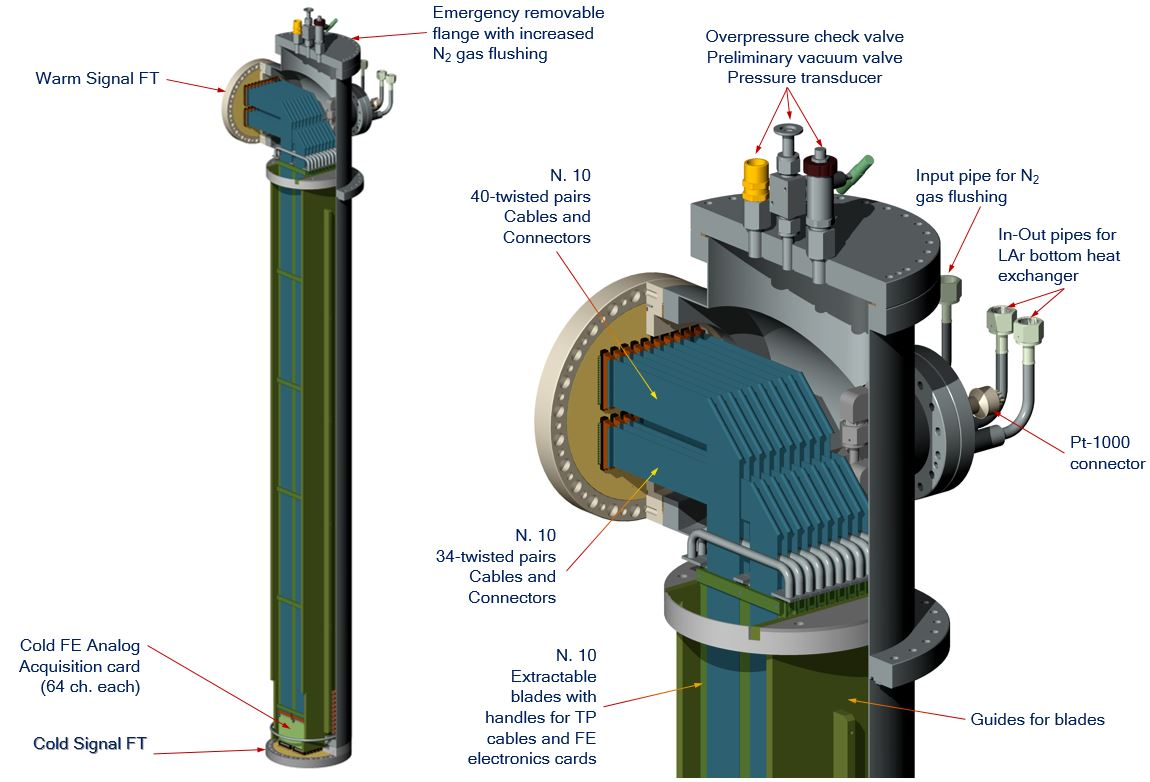
\includegraphics[width=0.8\textwidth]{dpele-sft-chimney-design}
\end{dunefigure}

The chimneys are closed at the bottom and top with vacuum-tight \fdth flanges whose function is to dispatch the signal and slow control lines. The \fdth at the bottom, the cold (signal) \fdth, isolates (ultra-high vacuum tightness standard) the inner volume of the \dword{dpmod} from the chimney volume and interconnects the signals from the \dword{crp} to the analog \dword{fe} cards. The \fdth at the top, the warm (signal) \fdth, seals the chimney from the outside environment. It also passes the low voltage and control lines to the \dword{fe} electronics inside and brings out the differential analog signal lines from the \dword{fe} amplifiers. 

The \dword{sftchimney} volume is filled with nitrogen gas at near-atmospheric pressure. The temperature inside the chimney can be adjusted using a heat exchanger copper coil cooled with \lar. It is located at the bottom close to the cold \fdth around the \dword{fe} cards. %The functions of 
This cooling system %are to 
mitigates the heat input to the main \dword{dpmod} volume and provides an optimal (lowest noise) operating temperature for the \dword{fe} electronics of around \SI{110}{K}. A pressure release valve, indicated in Figure~\ref{fig:dpele-sft-chimney-design}, protects the structure from an accidental overpressure in the inner volume. 

The expected heat input from a given \dword{sftchimney} is about \SI{20}{\watt}. This number includes the heat through the twisted-pair cables connected to the warm \fdth, the heat in the  \dword{sft} outer metallic tube, as well as the heat dissipation by the \dword{fe} cards. A total heat input from all \num{240} \dwords{sftchimney} is at the level of \SI{5}{\kilo\watt}. 

\begin{dunefigure}[\dword{sft} chimney cold flange]{fig:dpele-sft-cold-pcb}
{\dword{sftchimney} cold \fdth flange with one of the \dword{fe} cards mounted.}
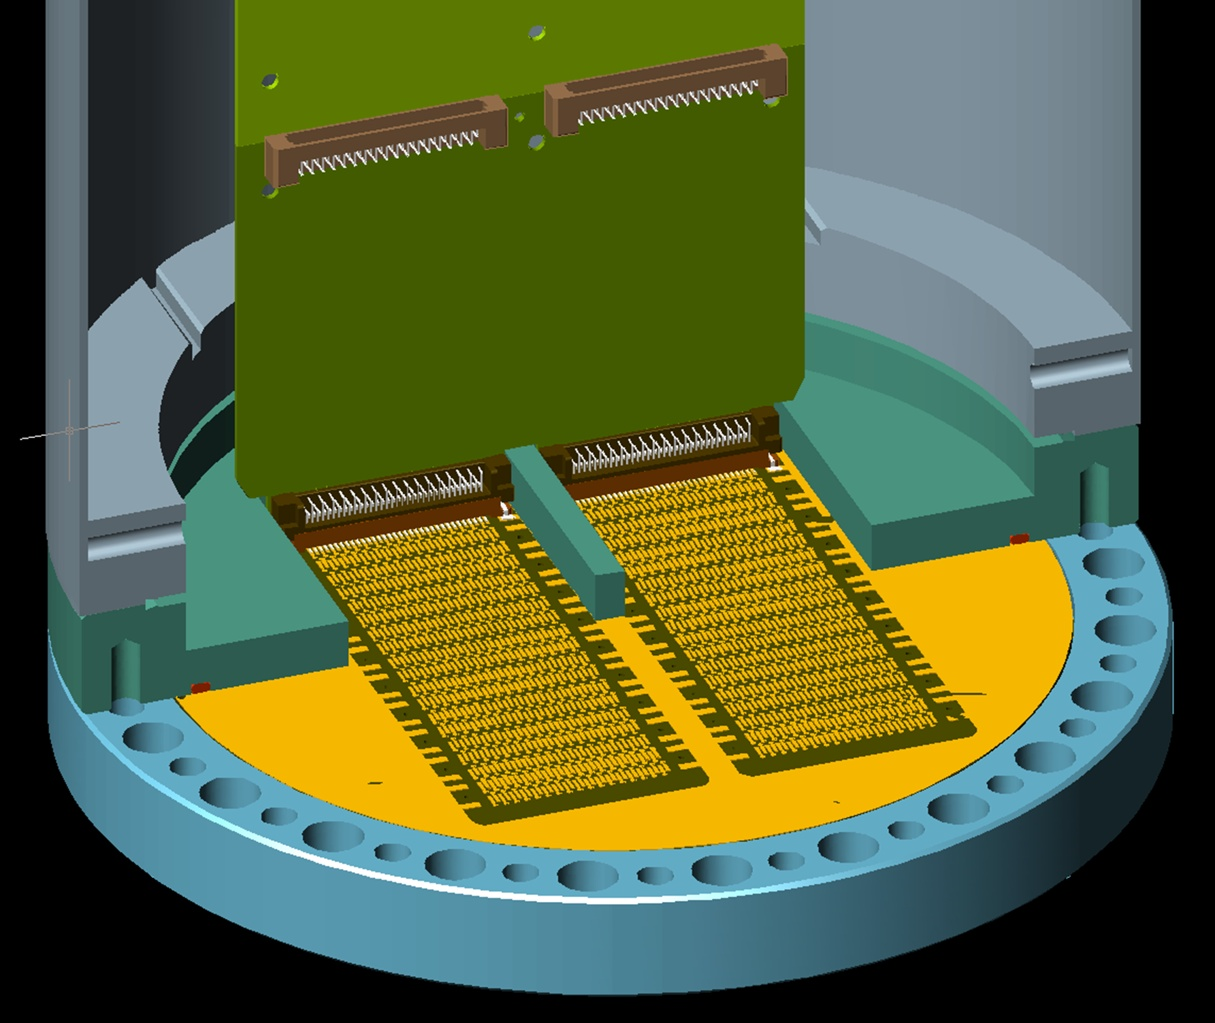
\includegraphics[width=0.6\textwidth]{dpele-sft-cold-pcb}
\end{dunefigure}
%%%%%%%%%%%% anne to here 4/13
The analog \dword{fe} cards are inserted directly onto the PCB of the cold \fdth of \dword{sftchimney}
%\fixme{same as \dword{sft}?} DONE
(see Figure~\ref{fig:dpele-sft-cold-pcb}). The other side of the PCB (facing inside the cryostat) hosts the connectors for the flat cables coming from the \dword{crp} anodes.  The \dword{fe} cards are mounted on \SI{2}{\m} long blades made from FR4 that enable the insertion and extraction of the electronics, and also support the flat cables carrying signals, low voltages, and slow control to and from the warm flange interface.  The blades slide along the rails installed inside the chimney at opposite sides; %which 
these rails guide the \dword{fe} cards to their respective connectors on the cold \fdth. 

Prior to the commissioning of a \dword{dpmod}, the chimneys are evacuated via a dedicated ISO standard KF16 port (see Figure~\ref{fig:dpele-sft-chimney-design}) and then filled with nitrogen gas. This ensures the removal of % the 
any moisture that would otherwise condense around the \dword{fe} cards, once the \dword{dpmod} is filled with the \lar, damaging the electronics. To access the \dword{fe} cards once the \dword{dpmod} is cold, the stainless steel flange at the top of the \dword{sftchimney} (Figure~\ref{fig:dpele-sft-chimney-design}) must be removed. This procedure requires continuous flushing of nitrogen gas at slight over-pressure (with respect to atmospheric) in order to prevent the humid air entering. % and generating condensation inside the chimney. 
Once a chimney is opened, it is possible to extract the blades with the \dword{fe} cards after unplugging the flat cables (two per card) connected on the inner side of the warm flange (Figure~\ref{fig:dpele-sft-chimney-design}).

The procedure to access the \dword{fe} cards under cold operation was successfully tested during the operation of the \dword{wa105} detector. The %temperature at the 
top of the chimney was very close to room temperature, allowing manipulation of the cable connections on the warm \fdth flange without %any 
cryogenic gloves. The movement of the blades on the rails and the \dword{fe} card extraction and insertion did not indicate any mechanical problems %that could have been caused by 
due to the shrinking of various elements % due to the 
at lower temperatures.  The signals from the \dword{fe} cards that underwent %the extraction/insertion 
this process were also checked and %no malfunctioning channels were found.
all channels functioned properly.

%%%%%%%%%%%%%%%%%%%%%%%%%%%%%%%%%%%
%\subsection{Low-voltage Power Supplies for \dword{fe} Electronics}
%\label{sec:fddp-tpc-elec-design-lvps}

%%%%%%%%%%%%%%%%%%%%%%%%%%%%%%%%%%%
\subsection{Digital Advanced Mezzanine Card Electronics for Charge Readout}
\label{sec:fddp-tpc-elec-design-amc}
%THIS IS CHARGE READ OUT
The %function of the
 \dword{cro} \dword{amc} cards % is to 
 read and digitize the data from the \dword{fe} amplifiers and %then 
 transmit them to the \dword{daq} system. The cards also include a last stage of analog shaping before the \dword{adc} input. The analog \dwords{fe} produce differential unipolar signals defined with respect to a baseline offset. 
% This offset is removed and the signals are subtracted in the analog input stage of the digital electronics prior to the digitization. 
Prior to the digitization, this offset is removed and the signals are subtracted in the analog input stage of the digital electronics.
Each card has eight \dword{adc} chips (Analog Devices, AD9257\footnote{Analog Devices\texttrademark{}, 
 \url{http://www.analog.com/media/en/technical-documentation/data-sheets/AD9257.pdf}.}, Table~\ref{tab:dpele-adc9257}), two dual-port memories (Integrated Device Technology IDT70T3339\footnote{Integrated Device Technology\texttrademark{} (IDT), \url{https://www.idt.com/document/dst/70t33391999-data-sheet}.}), and an \dword{fpga} 
 (Alterra\footnote{Alterra\texttrademark{}, \url{https://www.altera.com/products/fpga/cyclone-series/cyclone-v/overview.html}.} Cyclone V) on board. The \dword{fpga} provides a virtual processor (NIOS) that handles the readout and the data transmission. The choices for all of the components have been optimized with respect to the design requirements and technical criteria such as costs, chip footprint (small enough to fit on the \dword{amc}), power consumption, and ease of use (available functionality). 

\begin{dunetable}
[Main characteristics of \dword{adc} AD9257]
{lr} {tab:dpele-adc9257}
{Main characteristics of \dword{adc} AD9257.}
Item &   \\ \toprowrule
Channels & \num{8} \\ \colhline
Sampling & up to \SI{40}{MSPS} \\ \colhline %/\SI{65}{MSPS}
Resolution & \SI{0.122}{\milli\volt} \\ \colhline
Dynamic range & \num{14} bit/ \SI{2.0}{\volt} \\ \colhline
Differential non-linearity & typical \num{\pm0.6} LSB\\ 
& with min. \num{-1.0} and max. \num{+1.7} LSB  \\ \colhline
Integral non-linearity & typical \num{\pm1.1}  LSB\\
& with min. \num{-3.1} and max. \num{+3.1} LSB  \\ 
\end{dunetable}
%\fixme{what's LSB (in table)?} STANDARD TERM FOR DIGITAL ELECOTRONICS REFERRING TO THE LEAST SIGNIFICANT BIT

\begin{dunefigure}[Block diagram of \dword{amc}]{fig:dpele-amc-scheme}
{Block diagram of \dword{amc}.}
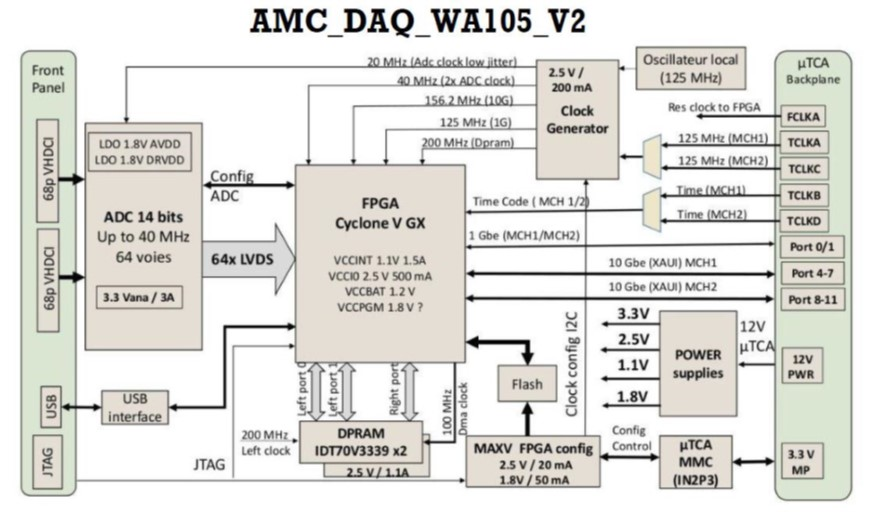
\includegraphics[width=0.9\textwidth]{dpele-amc-scheme}
\end{dunefigure}
Figure~\ref{fig:dpele-amc-scheme} shows block diagram of the \dword{amc} functionality. Each \dword{amc} generates a continuous compressed stream of \SI{2.5}{MSPS} \num{12}\,bit data per readout channel. The on-board ADCs operate at a rate of \SI{25}{\MHz} per channel. The data are down-sampled in the \dword{fpga} to \SI{2.5}{\MHz} by performing ten-sample averaging, which leads to further digital filtering of the noise. The data, consisting of only the  \num{12} most significant bits from each digitized \num{14}\,bit sample, are then compressed using an optimized version of the Huffman algorithm and organized in frames for transmission.  The frames contain the absolute timing information of the first data sample for reliability purposes. In the current design, each \dword{amc} has \num{64} channels and reads one analog \dword{fe} card.

The \dwords{amc} are housed in \dword{utca} crates and send their data via the \dword{mch} switch. The timing synchronization of \dwords{amc} is achieved via a \dword{wrmch} module (also housed in the crate) that is connected to the \dword{wr} network. In addition, a  \dword{wrmch} could also be used for triggered readout of \dwords{amc} by sending it dedicated packets containing trigger timestamp information over the \dword{wr} network.

In \dword{pddp}, \dwords{amc} are operated in the triggered mode, reading a \SI{4}{\milli\second} drift time window at a trigger rate of \SI{100}{Hz}, which is not far from %a 
continuous readout mode. The analog data are continuously digitized and buffered. It is possible to acquire a sub-sample of these data %can then be acquired 
by providing \dword{amc} with a timestamp generated by an external trigger. The timestamp defines the start time for the data sequence to be read, while the length of the sequence is determined by the size of the drift window. In \dword{pddp} this length corresponds to \num{10000} \SI{400}{\nano\second} samples per full drift window (\SI{4}{\milli\second}). 
%\fixme{not clear how the \num{10000} helps define the length; you say it's determined from the drift window size; clarify} DONE
 Triggers (beam counters, cosmic-ray counters, \dwords{pmt} detecting the UV light, and starts of beam spills) are time stamped in a dedicated \dword{wr} slave node (\dword{wr}-TSN), an FMC-DIO mezzanine mounted on \dword{wr} SPEC carrier card, which runs a custom firmware and is hosted in a computer. The \dword{wr}-TSN is connected to the \dword{wrgm} for synchronization and for transmission of the trigger information. The timestamp data produced by the \dword{wr}-TSN are sent over the \dword{wr} network as Ethernet packets with a customized protocol. 

%%%%%%%%%%%%%%%%%%%%%%%%%%%%%%%%%%%
\subsection{Electronics for Light Readout}
\label{sec:fddp-tpc-elec-design-lro}
%\fixme{section title: ``Digital'' Electronics for Light Reaout, in parallel with prev section?} THE ELECTRONICS INCLUDES CATIROC \dword{asic} WITH SOME ANALOG FUNCTIONALITY SO THE TITTLE SHOULD BE MORE GENERAL 
%
The \dword{lro} card is a \num{16} channel \dword{amc} containing one \num{16} channel \num{14} bit \SI{65}{\MHz} \dword{adc} (AD9249) and one \dword{catiroc} \dword{asic}. A block diagram of the prototype board used for \dword{pddp} is shown in Figure~\ref{fig:dpele-lro-scheme} and a photo in Figure~\ref{fig:dpele-lro-proto} . In this prototype a mezzanine board containing the \dword{asic} and \dword{adc} sits on a commercial mother board (Bittware S4 \dword{amc}\footnote{Bittware\texttrademark{}, Inc., \url{https://www.bittware.com/fpga/intel/boards/s4am/}.}) with a high specification \dword{fpga} (Alterra\footnote{Alterra\texttrademark{}, \url{https://www.altera.com/products/fpga/stratix-series/stratix-iv/overview.html}.} Stratix IV). In the final implementation for the \dword{dpmod}, the mezzanine is integrated with the layout of the \dword{amc} board developed for the charge readout.  
A proposed upgrade is a \num{32} channel card, %diminishing 
which would reduce the number of cards required and increase the channel density to \num{352} channels per \dword{utca} crate.

\begin{dunefigure}[Block diagram of \dword{lro}]{fig:dpele-lro-scheme}
{Block diagram of \dword{lro} prototype.}
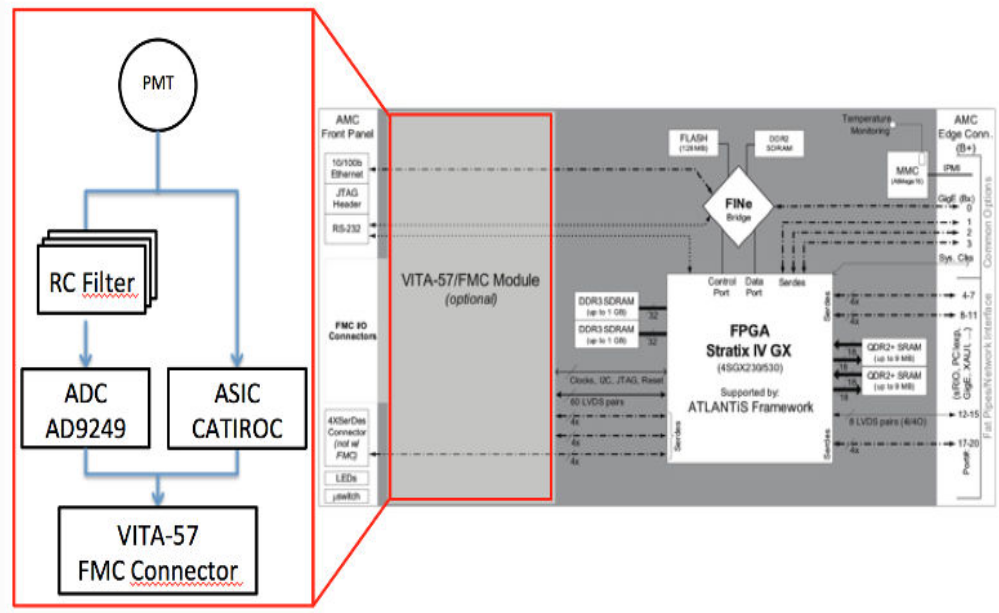
\includegraphics[width=0.8\textwidth]{dpele-lro-scheme}
\end{dunefigure}

\begin{dunefigure}[Photo of prototype \dword{lro} card]{fig:dpele-lro-proto}
{A photo of the \dword{lro} prototype.}
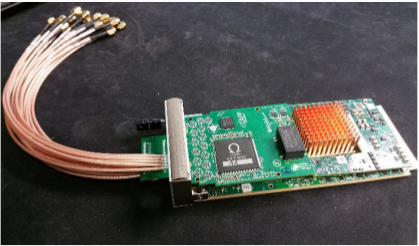
\includegraphics[width=0.7\textwidth]{dpele-lro-proto}
\end{dunefigure}

The analog signals from each \dword{pmt} channel are split equally into two separate branches (see Figure~\ref{fig:dpele-lro-scheme}) . One path (waveform branch), through an anti-aliasing low-pass filter and the \num{14} bit \SI{65}{\MHz} \dword{adc} (AD9249), produces continuous digitization of the \dword{pmt} waveform data, which are down-sampled to \SI{2.5}{MHz} prior to the transmission to \dword{daq}. The other (\dword{catiroc} branch) is routed directly to the \dword{catiroc} \dword{asic} for precise measurements of pulse charge and timing. Both paths produce data continuously and independently.

%%%%%%%%%%%%%%%%%%%%%
\subsubsection{Waveform branch} %\dword{adc}
%details on \dword{catiroc}
The main characteristics of the \dword{adc} used for continuous digitization of the \dword{pmt} signals are shown in Table \ref{tab:dpele-adc9249}.
%\rms and \dword{pmt} gain?
\begin{dunetable}
[Main characteristics of \dword{adc} AD9249]
{lr} {tab:dpele-adc9249}
{Main characteristics of \dword{adc} AD9249.}
Item &   \\ \toprowrule
Channels & \num{16} \\ \colhline
Sampling & \SI{65}{MSPS} \\ \colhline
Resolution & \SI{0.122}{\milli\volt} \\ \colhline
Dynamic range & \num{14} bit/ \SI{2}{\volt} \\ \colhline
Differential non-linearity & typical \num{\pm0.6} LSB\\
& with min. \num{-0.9} and max. \num{+1.6} LSB  \\ \colhline
Integral non-linearity & typical \num{\pm0.9}  LSB\\
& with min. \num{-3} and max. \num{+3} LSB  \\ 
%MEMORY??
\end{dunetable}
%noise llevel??

For normal operation, in the continuous mode, the digitized signals are down-sampled by the \dword{fpga} to a coarse \SI{400}{ns} sampling to match that of the \dword{cro} and limit the quantity of data streamed. 
%\fixme{is there a way to get rid of at least one or two instances of ``sample'' in the prev sentence?} DONE
The use of a higher specification \dword{adc}, with time-sampling of \SI{15.4}{ns}, allows for greater flexibility. % It is envisaged that 
For particular calibration runs, waveforms with finer time sampling could be read-out, allowing studies of, e.g., the \lar scintillation time profiles. %Even 
%During normal operation, as well, online pulse processing is possible within the \dword{fpga} using the finer time-sampled waveforms (before the down sampling), which could be used to make continuous measurements such as the rise and fall times of the pulses. 
During normal operation, as well, online pulse processing is possible within the \dword{fpga} using the finer time-sampled waveforms (before the down sampling; this would enable continuous measurements of quantities such as the rise and fall times of the pulses. Even at the coarse sampling rate of \SI{400}{ns}, studies of the \lar scintillation time profile are possible (given the long fall-time constant of $\sim$\SI{1500}{ns}) %and also 
as is matching of the electroluminescence signal (also known as proportional scintillation light) to that of the charge signal.  Low light-level signals, %such as the 
as from single or a few \phel{}s, % signals, 
will show no time structure, but will consist of one sample several LSB above the baseline. 

%%%%%%%%%%%%%%%%%%%%%
\subsubsection{CATIROC branch} %{Analog Measurements of Charge and Time}%\dword{asic}?

The \dword{catiroc} is a \num{16} channel \dword{asic} dedicated to measurement of charge and precision timing of negative-polarity \dword{pmt} signals~\cite{Blin:2017}. It auto-triggers on single \phel{}s and can sustain a high dark rate of up to \SI{20}{kHz/channel}. Charge measurements are possible over the range of \SI{160}{fC} to \SI{70}{pC} (corresponding to approximately to a range of \numrange{1}{400} \phel{}s with a \dword{pmt} gain of \num{1E6}). Timing measurements per channel can %be made with 
reflect an accuracy of \SI{200}{ps}.

\begin{dunefigure}[\dword{catiroc} \dword{asic}]{fig:dpele-lro-catiroc}
{Functional diagram of \dword{catiroc} \dword{asic}.}
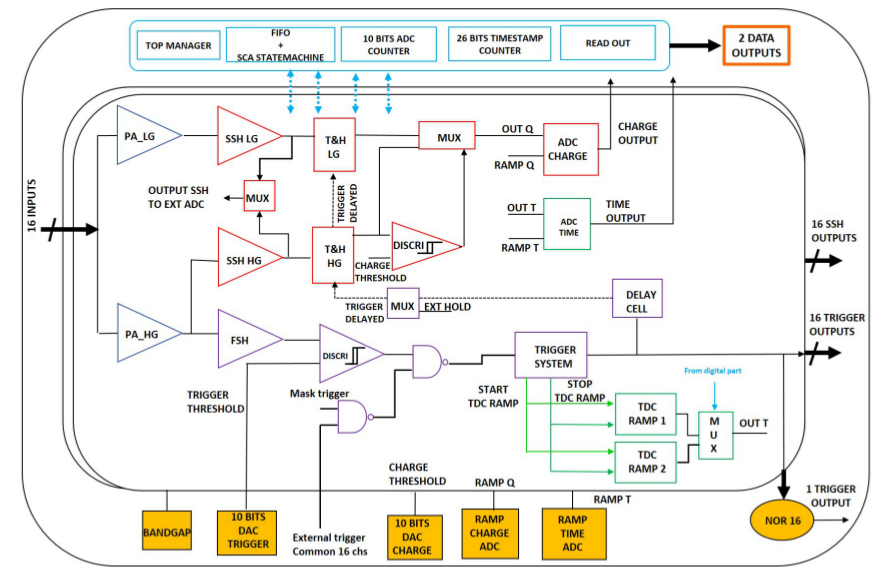
\includegraphics[width=0.8\textwidth]{dpele-lro-catiroc}
\end{dunefigure}

Figure~\ref{fig:dpele-lro-catiroc} shows the schematic of the \dword{catiroc} \dword{asic}. Its main properties are summarized in Table~\ref{tab:dpele-catiroc}. The slow channel, from which precision charge and timing measurements are made, is formed by two variable-gain (\SI{8}{bit}) amplifiers followed by two variable slow shapers; one high gain for small signals, and one low gain for larger signals, and two track-and-hold stages. The slow shaper has a tunable shaping time (up to \SI{100}{ns}) and a variable gain.  If the high gain is saturated, corresponding to passing a predetermined threshold common to all \num{16} channels, the lower gain value is chosen. The chosen charge value is converted by an internal 10-bit Wilkinson \dword{adc} operating at \SI{160}{MHz}.  This slow channel operates in a ping-pong mode, with two capacitors to store the slow shaper signals, giving an effective buffer of 2 events. If both capacitors are full, a deadtime of \SI{5}{\micro\second} arises.

\begin{dunetable}
[Main characteristics of \dword{catiroc}.]
{lr} {tab:dpele-catiroc}
{Main characteristics of \dword{catiroc}.}
Item &   \\ \toprowrule
Number of channels & \num{16}\\ \colhline
Signal polarity & negative \\ \colhline
Timing & Timestamp: 26 bit counter at \SI{40}{MHz} \\
       & Fine time: resolution $<$\SI{200}{ps}\\ \colhline
Charge Dynamic Range & \SI{160}{\femto\coulomb} to \SI{100}{\pico\coulomb}\\ \colhline
Trigger & auto-trigger \\
        & Noise = \SI{5}{fC} Minimum threshold = \SI{25}{fC} (5$\sigma$)\\ \colhline
Digital & 10-bit Wilkinson \dword{adc} at 160 MHz \\ %TWO READOUT AT 80MHZ??
        & Read-out frame of 50 bits \\ \colhline
Outputs & \num{16} trigger outputs \\
        & NOR16 \\
        & \num{16} slow shaper outputs \\
        & Charge measurement over \num{10} bits \\
        & Time measurements over \num{10} bits \\ \colhline
Main Internal &  Variable preamplifier gain \\
Programmable  &  Variable shaping and gain \\
Features & Common trigger threshold \\
         & Common gain threshold \\ 
\end{dunetable}

The fast channel is used to auto-trigger the \dword{asic} and make the fine-timing measurement. It comprises a high gain preamplifier, fast shaper (shaping time \SI{5}{ns}) and discriminator with a \num{10} bit programmable threshold that is common to all \num{16} channels. The output of the discriminator is used for the two time-to-digital convertors to get the fine timing. A coarse timestamp could also be obtained from a \num{26} bit counter running at \SI{40}{MHz}.  Only the data from the triggered channels are digitized; their information is transferred to the internal memory, which is read by the external \dword{fpga}. 

  
%%%%%%%%%%%%%%%%%%%%%%%%%%%%%%%%%%%
\subsection{Network-based $\mu$TCA Architecture}
\label{sec:fddp-tpc-elec-design-utca}

The digital electronics is based on \dword{utca} standard which offers an industrial solution with a very compact and easily scalable architecture to handle a large number of channels at low cost.  The standard (or related standards such as \dword{atca} or xTCA) is widely used in the telecommunication industry and is being adopted by the HEP community. The backplane of the \dword{utca} crates host high-speed serial links that support a variety of transmission protocols (Ethernet, PCI Express, SRIO, etc.). In addition, dedicated lanes are available for the distribution of the clock signals to all the boards hosted in the crate.  The Ethernet-based solution has been adopted for both the data and clock distribution in this design of the \dual electronics system for both charge and light readout (\dword{cro} and \dword{lro}. 

Each \dword{amc} for either charge or light readout plugged into the \dword{utca} is connected to the crate \dword{mch} board through the backplane serial links. The \dword{mch} provides the switch functionality that enables \dwords{amc} to communicate with each other or external systems through the \dword{mch} uplink interface. In the \dual electronics system design, \dword{mch} also manages the WR clock distribution. 

\begin{dunetable}
[Bandwidth requirements per $\mu$TCA crate.]
{lr}{tab:dp-utcabandwidth}
{Bandwidth requirements per \dword{utca} crate for continuous data streaming. A compression factor of 10 for the charger readout data is assumed }   
Parameter & Value  \\ \toprowrule
  \dword{cro} data rate  &  \SI{1.8}{Gibit/s}         \\ \colhline
  \dword{lro} data rate  &  \SI{4.7}{Gibit/s}            \\ \colhline
  Current \dword{mch} bandwidth & \SI{10}{Gibit/s}              \\ \colhline
  Upgradable \dword{mch} bandwidth & \SI{40}{Gibit/s}           \\ 
\end{dunetable}

In the current design, as used for \dword{pddp}, the \dword{mch} operates with a \SI{10}{Gbit/s} uplink. Given that a \dword{utca} crate hosts \num{10} \dwords{amc} for charge readout, the required bandwidth to stream the data to \dword{daq} is about \SI{1.8}{Gbit/s}. This assumes that the data exiting the \dwords{amc} are losslessly compressed with the compression factor \num{10}. The bandwidth required per crate link for streaming the \dword{lro} data is \SI{4.7}{Gbit/s}. The \SI{10}{Gbit/s} \dword{mch} is therefore sufficient to support these data rates. However, the technology is moving towards supporting the \SI{40}{Gbit/s} rates. In addition, the channel density per \dword{amc} could also be increased for cost optimization. For these reasons an upgrade to a \SI{40}{Gbit/s} \dword{mch} could be foreseen in the future. This would also imply that the optical links connecting the \dword{daq} system to \dword{utca} \dword{mch} should be operable at \SI{40}{Gbit/s}. A summary of the required and supported bandwidths per \dword{utca} crate for continous data streaming is provided in Table~\ref{tab:dp-utcabandwidth}.

\begin{dunefigure}[Instrumented \dword{utca} crate from the \dword{wa105}]{fig:dpele-311-utca-image}
{Pictures of an instrumented \dword{utca} crate from the \dword{wa105}. The crate contains five \dword{amc} cards, correspondingly to the number of readout channels per the \dword{sftchimney}. The images below show the crate after the  cables are connected to the warm flange of the \dword{sftchimney}.}
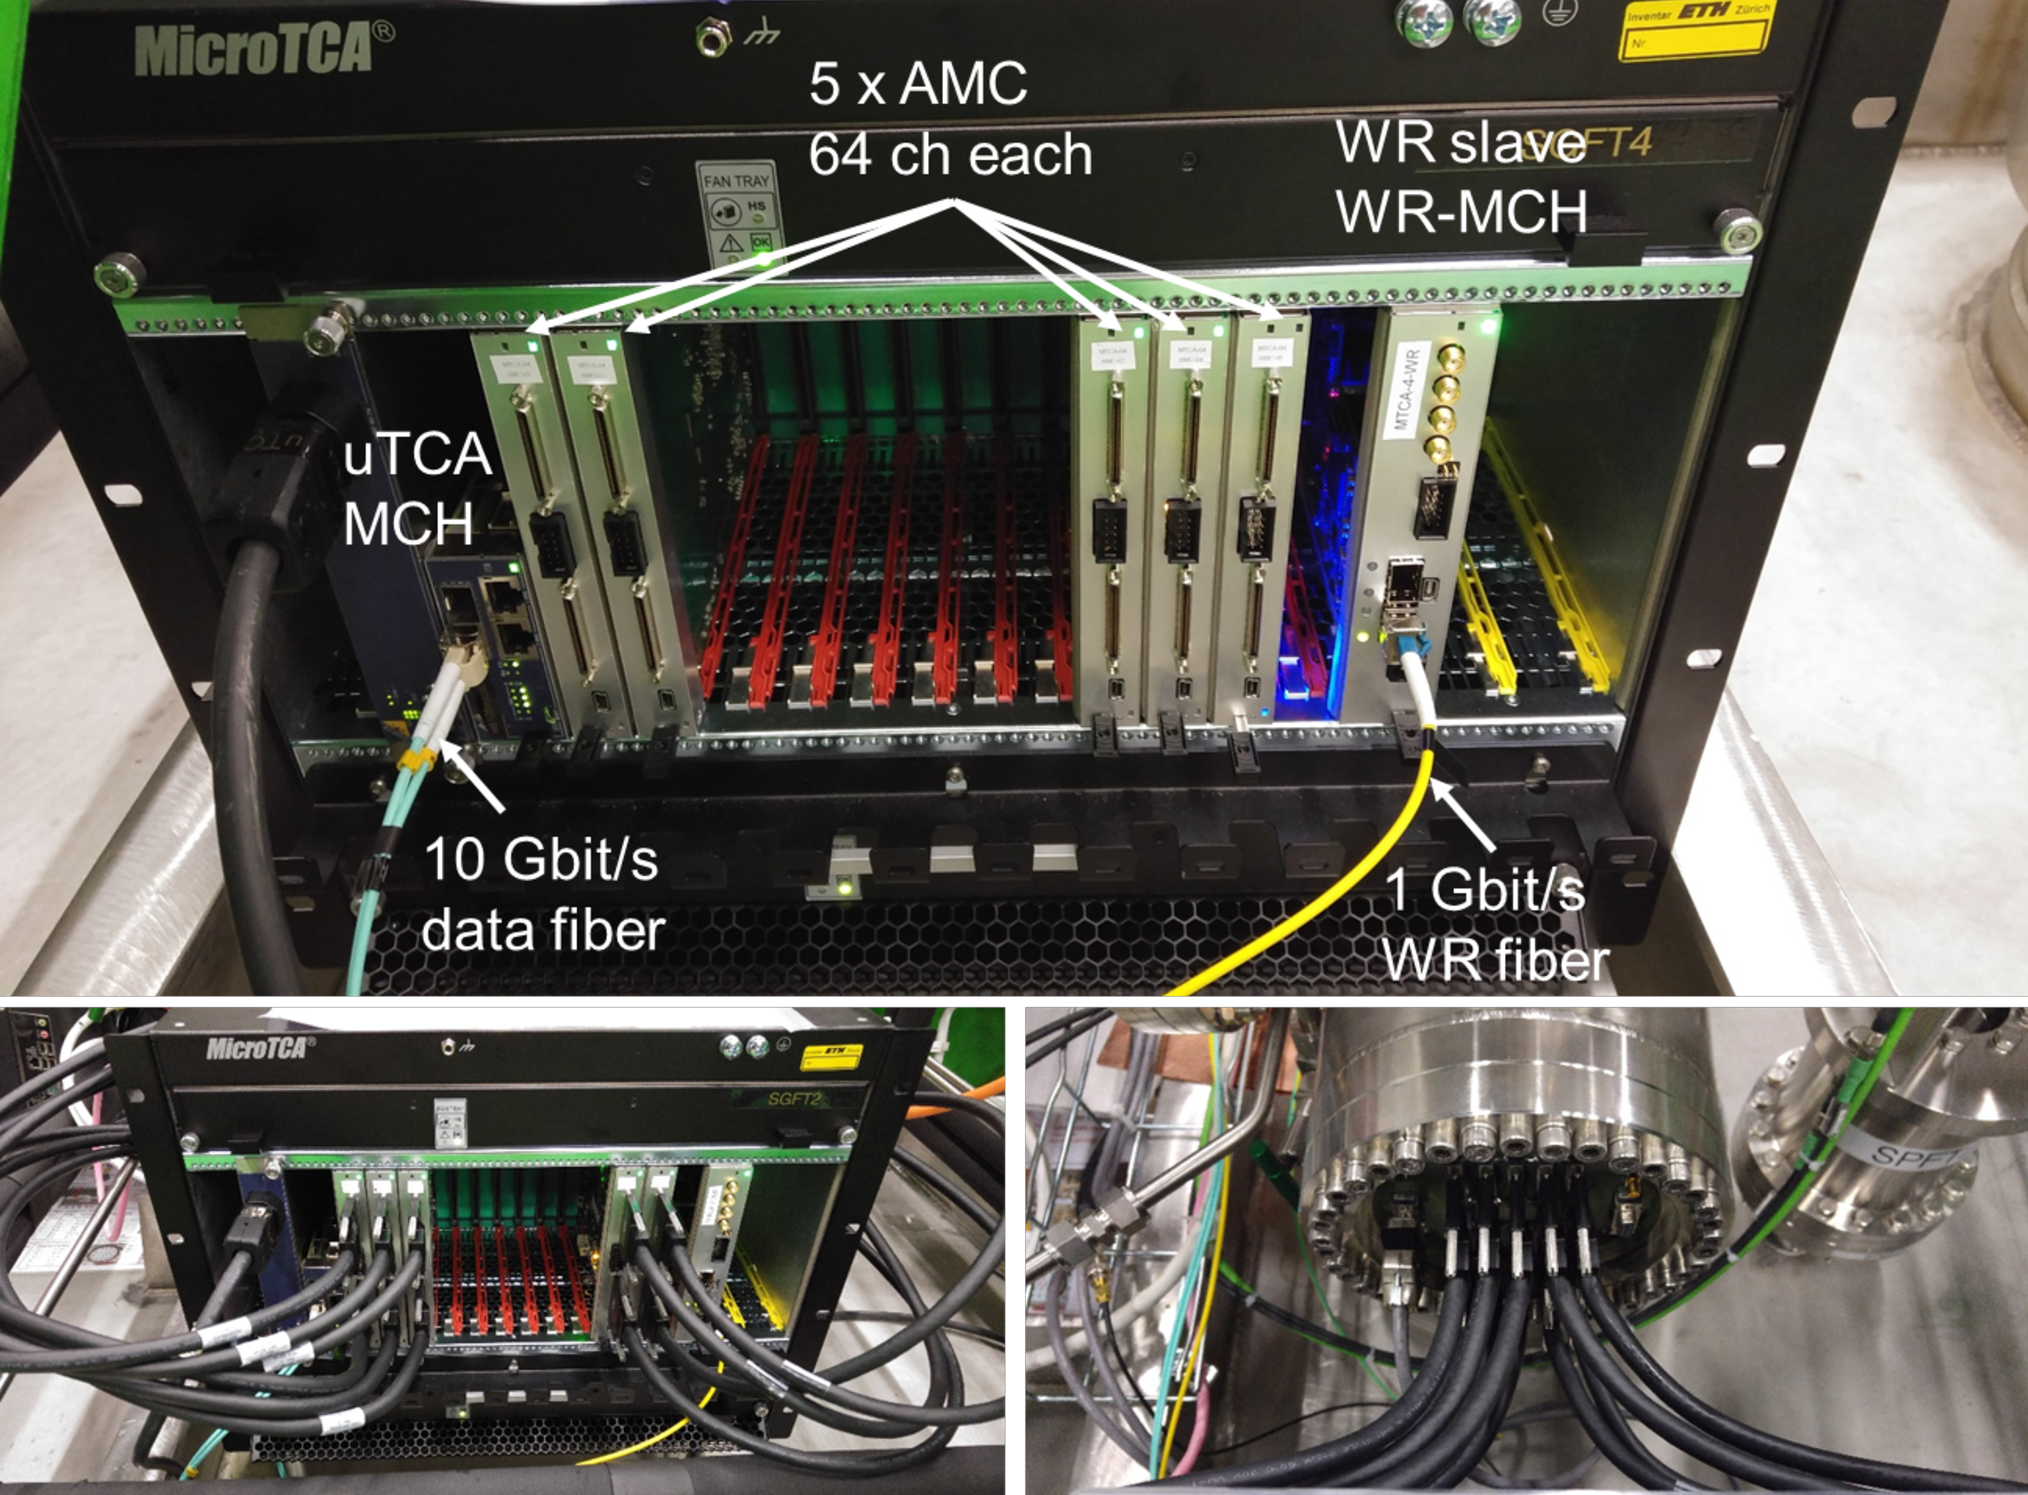
\includegraphics[width=0.6\textwidth]{dpele-311-utca-image}
\end{dunefigure}

As an illustration, Figure~\ref{fig:dpele-311-utca-image} shows pictures of one of the instrumented \dword{utca} crates used for the charge readout of the \dword{wa105} at CERN. In this detector each \dword{sftchimney} reads \num{320} channels, thus requiring only five \dwords{amc} per the \dword{utca} crate. The two optical fiber links, one (\SI{10}{Gbit/s}) for data and the other (\SI{1}{Gbit/s}) for clock and trigger timing distribution, are visible in the images.       

%%%%%%%%%%%%%%%%%%%%%%%%%%%%%%%%%%%
\subsection{Timing Distribution}
\label{sec:fddp-tpc-elec-wr}
% WR description and card development
The time synchronization system selected for the \dword{dpmod} utilizes a \dword{wr} network, which combines the synchronous \SI{1}{Gbit/s} Ethernet (SyncE) technology with the exchange of PTPV2 packets, to synchronize clocks of distant nodes to a common time. A high stability GPS disciplined oscillator (GPSDO) with  accuracy similar to that of an atomic clock provides a clock reference signal to be distributed over the physical layer interface of the \dword{wr} Ethernet network. The network topology is built using specially designed switches that have the standard IEEE802.1x Ethernet bridge functionality with an addition of \dword{wr}-specific extensions to preserve the clock accuracy. Time and frequency information are distributed to the nodes on the \dword{wr} network via optical fibers. The \dword{wr} protocol automatically performs dynamic self-calibrations to account for any propagation delays and keeps all connected nodes continuously synchronized to sub-ns precision. 

The sub-ns %accuracy 
precision on the clock synchronization is not strictly needed for aligning samples in the different \dword{amc} digitization units, since the %data have the timing granularity of 400 ns.
timing granularity on the data is \SI{400}{ns}. However, the \dword{wr} timing system offers readily available industrial components and the necessary protocols %needed 
for synchronization with automatic calibration of delay propagation. % and it, therefore, has been adopted. 
%This solution for the timing distribution was part of the R\&D started in 2006 and the final design for integrating this system with the readout of \dword{pddp} was completed in 2016.
R\&D on this timing distribution solution started in 2006; the final design for integrating this system, %foreseen for the \dword{dpmod}, the \dword{pddp} and the \dword{wa105} 
planned for the \dword{wa105}, \dword{pddp}, and the \dword{dpmod} readout, was completed in 2016. 
%\fixme{Is this relevant? what about timing of decision on using it for dp det module?} YES, THIS DEMONSTRATE THE STATE OF THE DESIGN READINESS

In the implementation specific to \dword{pddp}, a GPS-disciplined 
%fixme{`disciplined' seems a funny word here, but maybe that's what you call it?} YES THIS IS THE TERM USED FOR GPS TIMING SYSTEM (e.g., GPSDO)
clock unit (Meinberg LANTIME M600\footnote{Meinberg\texttrademark{}, \url{https://www.meinbergglobal.com/english/products/advanced-1u-ntp-server.htm}.}) feeds \SI{10}{MHz} and \num{1}\,PPS reference signals to a commercial \dword{wr} switch (Seven Solutions WRS v3.4\footnote{Seven Solutions\texttrademark{}, \url{http://sevensols.com/index.php/products/white-rabbit-switch/}.}). The switch acts as grandmaster of the \dword{wr} network. It is connected via \SI{1}{Gbit/s} optical links to the dedicated \dword{wr} timestamping node (\dword{wr}-TSN) and the \dword{wr} end-node slave cards present within each \dword{utca} crate (\dword{wrmch}) keeping these synchronized to its reference time. The \dword{wrgm} also communicates through a standard Ethernet port with the LANTIME unit for its date and time synchronization via NTP. The \dword{wr}-TSN module recieves analog TTL-level trigger signals, generates their timestamps, and transmits them over the \dword{wr} network to the connected \dword{wrmch} units. This timestamp information is then used by \dwords{amc} to find the data frame corresponding to the trigger. 

\begin{dunefigure}[Picture of \dword{wr} slave node card]{fig:dpele-wrmch-image}
{Picture of the \dword{wr} slave node card (\dword{wrmch}) present in each \dword{utca} crate for time synchronization.The \dword{wr}-LEN mezzanine card is visible in the bottom right corner.}
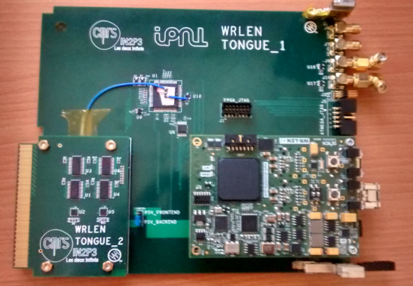
\includegraphics[width=0.45\textwidth]{dpele-wrmch-image}
\end{dunefigure}

The \dword{wrmch} card (Figure~\ref{fig:dpele-wrmch-image}) enables clock/timing/trigger distribution to \dwords{amc}. It communicates with them via dedicated lines in the backplane of the \dword{utca} crate using a customized data-frame protocol. The module contains a commercial WR slave node card, the \dword{wr} Lite Embedded Node (Seven Solutions OEM WR-LEN\footnote{Seven Solutions\texttrademark{}, \url{http://sevensols.com/index.php/products/oem-wr-len/}.}), as mezzanine card. WR-LEN runs on a customized firmware which also enables it to decode the trigger timestamp data packet received over the WR network.

\begin{dunefigure}[Architecture of \dword{wr} network]{fig:dpele-wrnet-layout}
{Architecture of WR network for time synchronization of digital readout electronics.}
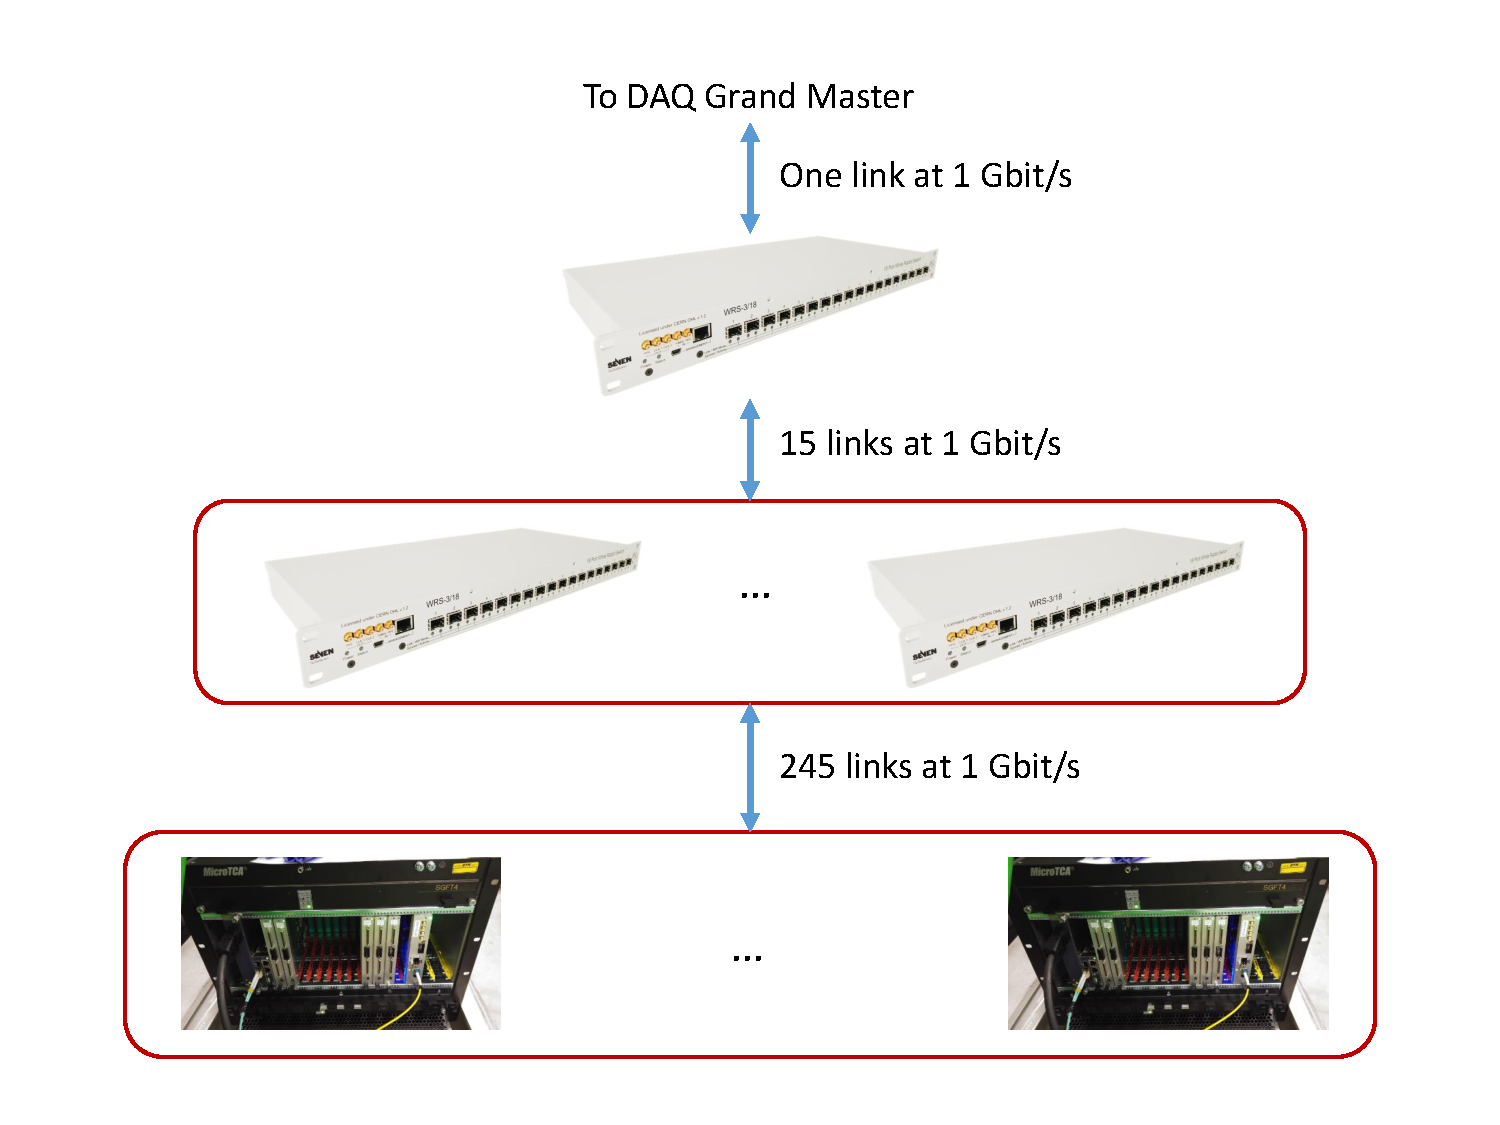
\includegraphics[width=0.8\textwidth]{dpele-wrnet-layout}
\end{dunefigure}

The architecture of the \dword{wr} network layout for one \dword{dpmod} is illustrated Figure~\ref{fig:dpele-wrnet-layout}. It is built in a hierarchical structure from \num{16} \dword{wr} switches with \num{18} ports each,  chained with \SI{1}{Gbit/s} optical fibers. The switch at the top of the hierarchy interconnects the synchronization %grand master
\dword{wrgm} from the \dword{daq} system with the \num{15} switches in the middle layer. These are in turn connected to the \dword{wrmch} slave nodes in each \dword{utca} crate (\num{245} in total for charge and light readout). 



%%%%%%%%%%%%%%%%%%%%%%%%%%%%%%%%%%%%%%%%%%%%%%%%%%%%%%%%%%%%%%%%%%%%
\section{Production and Quality Assurance}
\label{sec:fddp-tpc-elec-prod-assy}

%%%%%%%%%%%%%%%%%%%%%%%%%%%%%%%%%%
\subsection{Cryogenic Analog FE Electronics}
\label{sec:fddp-tpc-elec-prod-fe}
The production of the cryogenic \dwords{asic} and analog \dword{fe} cards is envisioned to be split between several sites located in France and Japan at the moment. The delivered cards are then split between five institutions in France (IPNL), Japan (KEK, NITKC, IU), and USA (SMU), where they are tested for various performance parameters such as noise levels, dead channels, hot channels, gain and its uniformity across channels, etc., at both room and operating cold temperature. An appropriate and common database will be developed and populated with test results. 
%\fixme{I don't think we want to list specific partners...} REQUESTED BY THE TC

%%%%%%%%%%%%%%%%%%%%%%%%%%%%%%%%%%
\subsection{Signal Feedthrough Chimneys}
\label{sec:fddp-tpc-elec-prod-sft}
A number of items require manufacture in order to produce the \dwords{sftchimney}. These include 
%The production of \dword{sft} chimneys consists of manufacturing 
\begin{itemize}
\item the PCB flanges for the warm and cold \fdth flange interfaces, 
\item the stainless steel pipe structure, 
\item the flanges containing the interfaces to the gas and liquid lines and slow control, 
\item the blades and railing, and 
\item the heat exchanger system. 
\end{itemize}
The flat cables that connect the \dword{fe} cards to the warm flange are commercially available products and are part of the \dword{sftchimney} procurement process. 
%\fixme{what stage? It hasn't been said} DONE

The %produced pieces 
manufactured components are delivered to %one or %several more
designated institutions participating in the \dual electronics consortium where teams verify the signal continuity %is verified 
for both cold and warm flanges, then assemble them into \dwords{sftchimney} and test for leaks. %The \dwords{sftchimney} are then assembled and tested for leaks. 
They also check the blade insertion, %is also checked 
 test the flat cables,  % are tested. The 
 then, once verified, pack the assembled \dwords{sftchimney} %are then packed 
 and ship them to SURF. 

%%%%%%%%%%%%%%%%%%%%%%%%%%%%%%%%%%
\subsection{The Timing System and $\mu$TCA}
\label{sec:fddp-tpc-elec-prod-utca}

The timing system components, the  \num{16} \dword{wr} switches and the \num{245} \dword{utca} crates containing the power modules, carrier hubs (\dword{mch}), and fan units,  %commercial components. 
are commercially available. The manufacturer takes the responsibility for the necessary quality control and quality assurance of these components, requiring no further testing on the part of the \dual electronics consortium. Once the components are delivered to the designated institutions, they can be sent to SURF for the installation. 

The commerical VHDCI signal cables (connecting the \dwords{amc} to the \dwords{sftchimney}) are procured and tested with the \dword{sftchimney} warm flanges.

%%%%%%%%%%%%%%%%%%%%%%%%%%%%%%%%%%
%\subsection{Low-voltage Power Supply System}
%\label{sec:fddp-tpc-elec-prod-lvps}

%%%%%%%%%%%%%%%%%%%%%%%%%%%%%%%%%%%
%\subsection{Digital Electronics}
%\label{sec:fddp-tpc-elec-prod-amc}

%%%%%%%%%%%%%%%%%%%%%%%%%%%%%%%%%%%
\subsection{Charge Readout Electronics}
\label{sec:fddp-tpc-elec-prod-cro}
The production of the \dword{amc} cards for the charge readout as well as the \dword{wrmch} slave cards for synchronization is currently shared between four institutions (IPNL, KEK, NITKC, IU). The cards ordered and delivered to each respective institution are subjected to quality assurance tests agreed upon by all participants.  
%\fixme{again, name particular institutions?}

%%%%%%%%%%%%%%%%%%%%%%%%%%%%%%%%%%%
\subsection{Light Readout Electronics}
\label{sec:fddp-tpc-elec-prod-lro}

The production of the \dword{lro} \dword{amc} cards is %currently envisaged to be made 
occurs in the same manner as the cards for \dword{pddp} since the number of cards to be produced and the channels to test are both small. The cards' electronic components, meeting required specifications, are purchased commercially. % to required specifications, for the production of the card. 
The project will be managed by a qualified engineer, working with a specialist in \dword{qa}.
%\fixme{working with?} DONE 

The produced cards are %first 
delivered to %the home institutes 
designated consortium institutions. %for testing before being shipped to the DUNE far site.  
%prior to shipment to SURF. %Basic quality tests are made upon delivery to ensure conformity of production; including visual inspection and electrical testing.
Upon delivery, teams conduct basic quality tests, including visual inspection and electrical testing, to ensure conformity of production. 
Another series of tests is performed on %each 
the cards to ensure their correct functionality and to evaluate their performance. Measurements include: linearity measurements (DNL and INL) of each \dword{adc} channel, and %tests of the 
linearity of response of the \dword{asic}. The level of cross-talk on the \dword{asic} %must also be 
is also quantified.

A dedicated single-channel setup, with \dword{pmt} (Hamamatsu R5912-02-mod), and identical cabling and splitter as in the \dword{fd}, can be used to characterize the expected noise level of each channel, and response to single \phel{}s up to saturation. 
Multiple cards are operated in a \dword{utca} crate with the %DUNE 
\dword{daq}.

After %shipping 
shipment to SURF and installation on-site, a small series of tests is performed with a pulse generator to verify the good working condition of the cards. Noise-level measurements are %also made as part of 
included in the integration effort.

%%%%%%%%%%%%%%%%%%%%%%%%%%%%%%%%%
%\subsection{Assembly Procedures}
%\label{sec:fddp-tpc-elec-assy}

%%%%%%%%%%%%%%%%%%%%%%%%%%%%%%%%%%%
%\subsection{Quality Assurance}
%\label{sec:fddp-tpc-elec-qa}


%%%%%%%%%%%%%%%%%%%%%%%%%%%%%%%%%%%%%%%%%%%%%%%%%%%%%%%%%%%%%%%%%%%%
\section{Interfaces}
\label{sec:fddp-tpc-elec-intfc}

%The \dword{dpmod} TPC electronics system has interfaces to several other systems. The system must read the charge and light signals from the \dword{dpmod} and thus needs to interface to \dword{crp} and the photo-detection systems.  The digitized data must in turn be transmitted to \dword{daq} via the optical links in each \dword{utca} crate. The \dwords{sftchimney} need to be integrated into the cryostat structure and connected to the cryogenic/gas  system. The management of the low-voltage power supplies for the \dword{fe} analog electronics and \dword{utca} crates as well as the monitoring of various sensors in the \dwords{sftchimney} have to be part of the slow control. The features of these interfaces are described here, while Table~\ref{tab:dpele-interfaces} provides the references to the relevant interface documents.

The \dual electronics system interfaces to several other systems, starting with the \dword{crp} and the \dword{pd} systems.  The digitized data must in turn %be transmitted 
flow to the \dword{daq} via the optical links in each \dword{utca} crate. The \dwords{sftchimney} integrate into the cryostat structure and connect to the cryogenics and gas systems. The slow-control system takes on management of the low-voltage power supplies for the \dword{fe} analog electronics and \dword{utca} crates, and  monitors various sensors in the \dwords{sftchimney}. %have to be part of the slow control. 
%The features of these interfaces are described here, while 
Table~\ref{tab:dpele-interfaces} provides the references to the relevant interface documents for each interface, stored in the DUNE document database (DocDB).

\begin{dunetable}
[Interface documents relevant to \dual TPC electronics system]
{lr}{tab:dpele-interfaces}{Interface documents relevant to \dual electronics system.}   
Interface document    & DUNE DocDB No. \\ \toprowrule
\dword{dp} TPC electronics to \dword{dp} \dword{crp} & 6751 \\ \colhline
\dword{dp} TPC electronics to \dword{dp} \dword{pd} & 6772 \\ \colhline
\dword{dp} TPC electronics to Joint \dword{daq} & 6778 \\ \colhline
\dword{dp} TPC electronics to Joint CISC & 6784 \\ \colhline
Facility Interfaces to \dword{dp} TPC electronics & 6982 \\ \colhline
Installation interfaces to \dword{dp} TPC electronics & 7009 \\ \colhline
Integration facility to \dword{dp} TPC electronics & 7036 \\ \colhline
Calibration to \dword{dp} TPC electronics & 7063 \\ \colhline
DUNE physics to \dword{dp} TPC electronics & 7090 \\ \colhline
Software and computing to \dword{dp} TPC electronics & 7117 \\ 
\end{dunetable}

%\fixme{Add in appropriate subsections for the pieces that TPC Electronics interfaces with. These initial ones may not be right.}

%%%%%%%%%%%%%%%%%%%%%%%%%%%%%%%%%%%
\subsection{Electronics System to \dword{crp} and Photon Detection Systems}
\label{sec:fddp-tpc-elec-intfc-crppmt}
%\fixme{clarify CRO vs LRO anne} CLARIFIED

The cold \fdth flange of the \dwords{sftchimney} forms the interface between the \dword{crp} and the \dword{cro} electronics system. On the side facing the cryostat the flange PCB has \num{20} \num{68}\,pin connectors (KEL 8930E-068-178MS-F\footnote{KEL Corporation\texttrademark{}, \url{https://www.kel.jp/english/product/product_detail/?id=490\&pageID=3\%20}.}) for plugging the flat cables from the \dword{crp}. These are \num{68}\,channel twisted-pair flat cables, each carrying signals from \num{32} anode strips and are within the scope of the \dword{crp} system. Each analog \dword{fe} card reads \num{64} anode strips, i.e., % implying receiving 
signals from two KEL connectors. The order in which the cables are connected %into 
to the cold flange determines the mapping of the electronic channels to the physical location of the strips on the \dword{crp} and is %should be 
coordinated carefully with the \dword{crp} consortium. %As an illustration, 
Figure~\ref{fig:dpele-sft-cold-flange} shows two images of the cold \fdth from the \dword{wa105}.
%%%%%%%%%  Anne to here EOB 4/16

\begin{dunefigure}[Images of the \dword{wa105} \dword{sft} cold \fdth]{fig:dpele-sft-cold-flange}
{Images of the \dword{wa105} \dword{sft} cold \fdth with the \dword{fe} cards inserted (right) and signal cables from \dword{crp} connected (left). The \dword{wa105} \dwords{sftchimney} read only \num{320} channels thus requiring \num{5} \dword{fe} cards.}
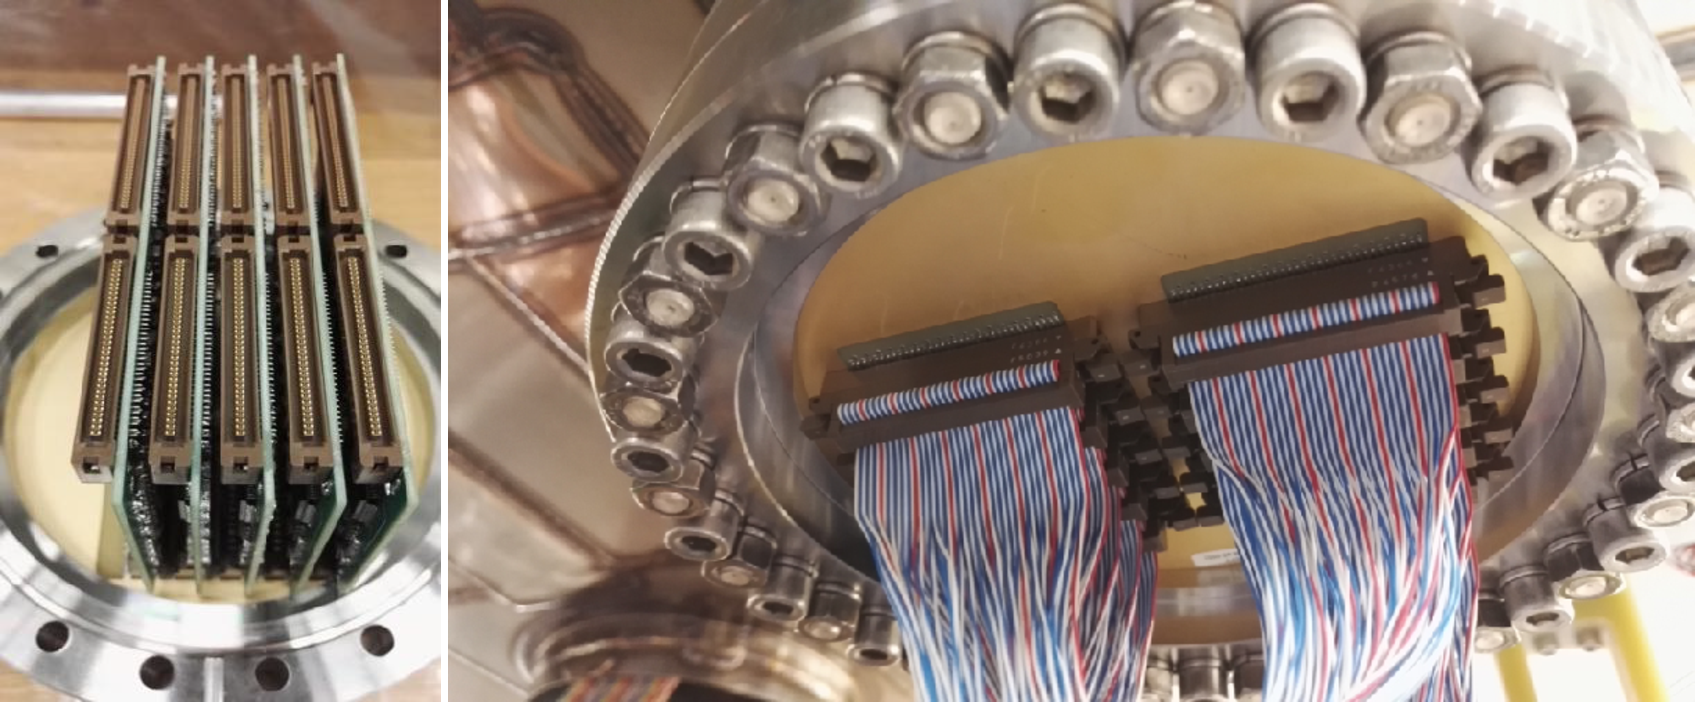
\includegraphics[width=0.8\textwidth]{dpele-sft-cold-flange}
\end{dunefigure}

The \dword{lro} electronics system is connected to the specific \dword{lro} signal \fdth flanges on top of the cryostat via coaxial cables, which are within the scope of the \dword{pds}.
The \dword{lro} electronics is designed for negative polarity \dword{pmt} signals, with the amplitude of single \phel{}s on the input of the card between \num{1} and \SI{10}{\milli\volt}. Assuming a typical \dword{pmt} gain of \num{1E6} (not accounting for attenuation of the signals), the Catiroc \dword{asic} can measure a range of \num{1} to \num{400} \phel{}s (\SI{160}{\femto\coulomb} to \SI{70}{\pico\coulomb}). The \dword{adc} samples from \SI{1}{\milli\volt} to \SI{1}{\volt} corresponding to \num{1} to \num{1000} \phel{}s, including the time response of the scintillator the range can increase to $\sim$\num{6000}. Increasing the gain of the \dword{pmt} to \num{1E7}, lowers the upper values by a factor of 10. The internal noise level of the \dword{catiroc} is below \SI{0.1}{\milli\volt}. The objective for the noise level of the \dword{adc} is for each channel to have the \rms noise level greater than \SI{0.5}{LSB}, aiming for \SI{1}{LSB} \SI{0.1}{\milli\volt}.
%at 65 MHz...
%\fixme{Why is this last bit of info under interfaces? I don't see anything about cables or connections; not needed? } ADDED A SENTENCE

%%%%%%%%%%%%%%%%%%%%%%%%%%%%%%%%%%%
\subsection{Electronics System to DAQ System}
\label{sec:fddp-tpc-elec-intfc-daq}

The hardware interface between the \dual \dword{cro} and \dword{lro} electronics sub-systems and \dword{daq} has two components. 
%\fixme{Same for \dword{crp} or PD electronics?} DONE
The first interface is the \SI{10}{Gbit/s} optical fibers for data transfer between the \dword{utca} crates and the network interface of the \dword{daq} system. The second one is a \SI{1}{Gbit/s} optical fiber that connects the \dword{daq} \dword{wrgm} switch to the \dual electronics timing system.   

In the current design 
%\fixme{we shouldn't be talking about baseline vs current (below), right? ``The design...''} DONE
a given \dword{dpmod} would have \num{245} \SI{10}{Gbit/s} optical links for streaming the digitized data to the \dword{daq} from the \dword{cro} (\num{240} links) and \dword{lro} (\num{5} links) electronics housed in \dword{utca} crates on top of the cryostat structure.  In the current specifications, the fibers are multimode OM3 fibers \cite{om3fibers} with LC-LC connectors suitable for the transmission over distances of up to \SI{300}{\metre}.  They are provided by the \dword{daq} consortium. On the side of the \dword{utca} crate, the fibers are connected to an optical transceiver in the \dword{mch} (two SFP+XAUI links) \cite{natmch}.  On the \dword{daq}, they go to the level-1 machines of the trigger farm, or switches, depending on the network topology adopted in the \dword{daq} system design.

The \SI{1}{Gbit/s} link going from the \dword{wrgm} to the \dual electronics time distribution network serves to provide the synchronization to the reference clock common for the entire FD and derived from a GPSDO %(GPS-Disciplined Oscillator) 
clock unit installed on the surface. The clock information is distributed to the \dword{wrmch} slave module in each \dword{utca} crate via a set of \dword{wr} switches. These switches and the interconnecting \SI{1}{Gbit/s} fibers form the timing sub-system of the \dual electronics system and are included in the design of the latter. The \dword{wr} synchronization protocol includes the automatic and continuous calibration of the propagation delays between the master and the connected slaves. This allows maintaining the overall synchronization between different nodes at sub-ns level. The \dword{wrgm} %could be possibly located 
will be located either:
\begin{itemize}
\item{On the surface near the GPSDO. In this case, a single fiber connects it to the \dual timing system underground. %The incurred latency due to the  necessary fiber length to deliver the timing signals underground is automatically taken into account by the system. 
The system automatically accounts for the incurred latency due to the extensive 
 fiber length.}
\item{Underground in the \dword{cuc}. In this case, calibration of the propagation delays between GPSDO and the \dword{wrgm} is performed manually, and a timing correction %would need be 
is applied to the data afterward.}
\end{itemize} 

The TPC electronics design assumes that the data are streamed continuously via the \SI{10}{Gbit/s} links to the \dword{daq}, where they are buffered until a trigger decision %could be 
is made. The triggers are to be issued by processing the buffered data in some suitable sliding time window on the trigger farm machines. 
%The depth of the window may go up to \SI{10}{s} as needed for the definition of the Supernova triggered events. 
The window may be as long as \SI{10}{s} for \dword{snb}-triggered events.
The triggers determine whether the data contained in the buffers are to be written on disk. 

The software interface between the \dword{daq} and the electronics system
%\fixme{sytem or systems?} DONE
includes the tools for handling the data transmission and buffering, i.e.,  data formatting in \dword{udp} packets, compression and decompression, and exchange of the control packets.

%%%%%%%%%%%%%%%%%%%%%%%%%%%%%%%%%%% to here noon Wed Anne
\subsection{Electronics System to Cryostat and Cryogenics}
\label{sec:fddp-tpc-elec-intfc-cryo}

The interface point between the cryostat and the \dual electronics system is at the cryostat penetrations where the \dwords{sftchimney} are %to be 
installed. Each penetration %should 
accommodates the chimney (of external diameter \SI{254}{\mm}). Each chimney has a CF-273 flange welded to its outer structure (see Figure~\ref{fig:dpele-sft-chimney-crosspipe}). After the chimney is inserted, this flange is in contact with the corresponding flange on the crossing (or penetration) pipe embedded in the cryostat structure to which it is eventually fastened. In order to avoid any leaks at this interface a CF-273 copper gasket is used to ensure the vacuum tightness.  

\begin{dunefigure}[Details of \dword{sftchimney} interface to the cryostat structure]{fig:dpele-sft-chimney-crosspipe}
{Details of \dword{sftchimney} interface to the cryostat structure.}
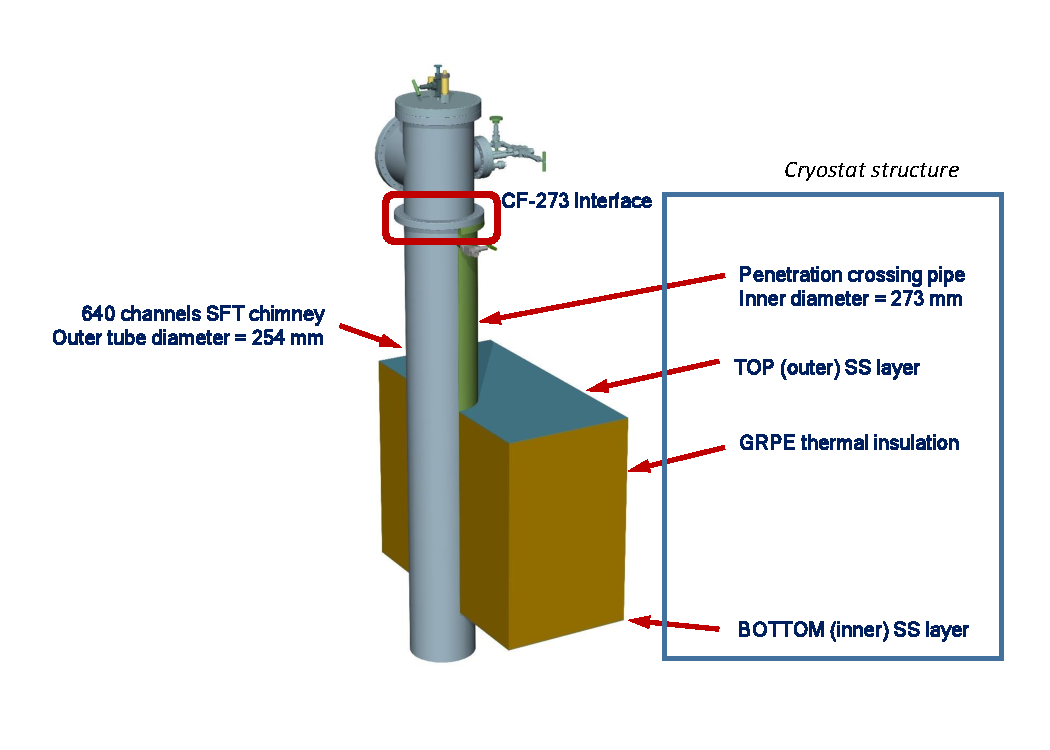
\includegraphics[width=0.7\textwidth]{dpele-sft-chimney-crosspipe}
\end{dunefigure}

Each chimney contains a heat exchanger copper coil cooled with \lar. There are two (inlet and outlet) stainless steel pipe connections with \SI{10}{\mm} and \SI{12}{\mm} inner and outer diameters, respectively, that need to be branched to the respective system for the \lar delivery and recirculation. In addition, %there is 
a connection for nitrogen gas line with the same pipe dimensions as those for the \lar cooling, %which 
is used for filling the chimney after it is closed following the installation of the \dword{fe} electronics. The nitrogen line is also required for flushing the chimney in the case of an access to the \dword{fe} cards after the \dword{dpmod} is cooled for the operation. 
%\fixme{does last sentence belong here?} IT PROVIDES CONTEXT FOR THIS PARTICAL PART OF THE SFT SYSTEM

The \dword{utca} crates for charge readout %need to be 
are installed within a short \SI{<0.5}{\meter} distance from the \dwords{sftchimney} on top of the cryostat roof. The five \dword{utca} crates for the light readout are also placed on the roof of the cryostat at optimal locations defined by the routing of the \dword{pmt} signal cables. The required volume to accommodate the crates is roughly \SI[product-units=power]{60x50x40}{\cm}. 

%%%%%%%%%%%%%%%%%%%%%%%%%%%%%%%%%%%
\subsection{Electronics System to Slow Control System}
\label{sec:fddp-tpc-elec-intfc-sc}

The integration with the slow control of the low-voltage power supply system for the \dword{fe} cards and \dword{utca} crates is required to enable the remote management and monitoring (current consumption by \dwords{asic}, set voltage, etc.). In addition, the \dwords{sftchimney} contain several sensors that need to be monitored. These include a pressure transducer that measures the pressure inside the chimney and at least two temperature probes (PT1000) that monitor the gas temperature inside near the cold flange at the bottom and close to the warm flange at the top. The readout of the \dword{utca} crate information and the sensors in the \dwords{sftchimney} is part of the Slow Control system.
%\fixme{specify who is responsible for what}

%%%%%%%%%%%%%%%%%%%%%%%%%%%%%%%%%%%%%%%%%%%%%%%%%%%%%%%%%%%%%%%%%%%%
\section{Transport and Handling}
\label{sec:fddp-tpc-elec-install-transport}
%\fixme{provide rough dimensions for boxes, chimney weights?}
%\fixme{specify that the chimneys are to be delivered for the installation underground and positioned around the cryostat on top.}

The \dwords{sftchimney} are \SI{2350}{\mm} long %objects with the weight of 
and weigh \SI{180}{\kg}.  The cold and warm flanges are mounted on them at the assembly site, and the chimneys undergo leak-testing prior to shipping in wooden crates (approximate dimensions \SI[product-units=power]{2.5x0.5x0.5}{m}). %, and arrive with the cold and warm flanges already mounted. 
Once at SURF the crates are moved underground and placed on the roof of the cryostat by the \dword{uit}. The %personnel from the 
\dual electronics consortium %then proceeds 
is then responsible for unpacking the crates and installing the \dwords{sftchimney}. The chimneys are delivered with the cold and warm flanges already mounted and and leak tested. %by one or several participating institutions.  
%\fixme{ I took out mention of ``one or several participating institutions'' Why not put that in section~\ref{sec:fddp-tpc-elec-design-sft}?}

The boxes containing the electronic cards and \dword{utca} crates are also handled by \dual electronics consortium personnel. These are expected to be lightweight and %could be easily carried. 
easy to carry. A box containing \num{100} \dword{amc} cards has a maximal dimesions of \SI{60}{\cm} and weighs less than \SI{10}{\kg}. 
% \fixme{transport info on the cards?}

%%%%%%%%%%%%%%%%%%%%%%%%%%%%%%%%%%%%%%%%%%%%%%%%%%%%%%%%%%%%%%%%%%%%
\section{Installation, Integration and Commissioning}
\label{sec:fddp-tpc-elec-install}

The installation of the TPC electronics systems proceeds in several stages. In order to cable the \dwords{crp} to the \dwords{sftchimney}, %these 
the chimneys 
%\fixme{check} %have to be 
are installed first, prior to the start of the \dword{crp} installation inside the cryostat. %After the chimneys are installed 
Next the \dword{fe} cards %could be 
are mounted on the blades and inserted. The installation of the digital electronics and \dword{utca} crates %should, however, be 
is postponed until all of the heavy work finishes on top of the cryostat in order to prevent %ensure that 
damage to the fragile components (e.g., optical fibers)  %are not accidentally damaged 
due to movement of material and traffic. %large traffic of personnel. 
Once the \dword{utca} crates are installed and all the digital cards are inserted, the %relevant 
\dwords{amc} are cabled to the warm flanges of the \dwords{sft} for the charge readout and are connected to the \dword{pmt} signal cables for the light readout. Finally, to complete the installation and integrate the system with the \dword{daq}, the \SI{10}{Gbit/s} and \SI{1}{Gbit/s} optical links to the \dword{daq} and \dword{wr} timing network are connected. At this stage the full system is ready for commissioning. 


%%%%%%%%%%%%%%%%%%%%%%%%%%%%%%%%%%%
\subsection{SFT Chimneys}
\label{sec:fddp-tpc-elec-install-sft}

The installation of the \dwords{sftchimney} requires a compact gantry crane with %the supports 
movable supports along the length of the cryostat. The crane itself moves along the transverse direction. The crates containing the \dwords{sftchimney} are placed along the edges of the cryostat roof. An unpacked chimney is hoisted and transported to %its respective 
the appropriate penetration crossing pipe for installation. Once in place, the chimney is fastened to the flange on the crossing pipe. %The length of each chimney is about \SI{2.4}{m}. 
Enough overhead room to accommodate a chimney's \SI{2.4}{m} length is required
%should therefore be foreseen 
to allow to free movement of the chimney with the crane along the direction transverse to the beam axis. 
%\fixme{why is transverse direction relevant here?} BECAUSE THERE IS NO CRANE IN THAT DIRECTION

In parallel with the \dword{sftchimney} installation, the \dword{fe} cards are unpacked on top of the cryostat and mounted on the blades prior to their insertion in the chimneys.  
% \fixme{Is this necessary: ``This work is performed on the roof of the cryostat to avoid repackaging the blades after the assembly in order to bring them on top of the cryostat.''?} 
With \dwords{sftchimney} secured in the cryostat structure, the blades with mounted \dword{fe} cards %can be inserted and the chimney can be sealed. 
are inserted prior to sealing the chimney.
%At this stage, the connections with the pipes for the \lar and gas nitrogen delivery could also be made, if these latter have already been installed. The pressure probes and temperature sensors can be connected to the slow control system.
At this stage, the \lar and gas nitrogen delivery pipes are already installed, and  
%\fixme{will the sequence be known?} THIS IS TO BE PROVIDED BY THE CRYOSTAT INFRASTRACTURE 
it is possible to make the connections with them. The pressure probes and temperature sensors are also connected to the slow control system.
 
 
%%%%%%%%%%%%%%%%%%%%%%%%%%%%%%%%%%%%
\subsection{Digital $\mu$TCA Crates}
\label{sec:fddp-tpc-elec-install-utca}

The installation of the \dword{utca} crates with the digital electronics %should happen 
takes place in the final stage of the \dword{dpmod} installation to avoid damaging the fragile equipment. The crates are placed in their designated positions on the cryostat and connected to the power distribution network. The \dword{amc} cards and \dword{wrmch} modules are inserted in their slots. The VHDCI cables are then attached connecting the \dword{cro} \dwords{amc} to the warm flange interface of the \dwords{sftchimney}.  The fibers from the timing system are connected to \dword{wrmch}. 

%%%%%%%%%%%%%%%%%%%%%%%%%%%%%%%%%%%%
%\subsection{Infrastructure}
%\label{sec:fddp-tpc-elec-install-cable}

%%%%%%%%%%%%%%%%%%%%%%%%%%%%%%%%%%%
%\subsection{Integration}
%\label{sec:fddp-tpc-elec-install-integ}

%%%%%%%%%%%%%%%%%%%%%%%%%%%%%%%%%%%
\subsection{Integration within the DAQ}
\label{sec:fddp-tpc-elec-install-daq}
The integration of the \dual TPC electronics with the \dword{daq} system requires connecting the \SI{10}{Gbit/s} fiber links to each of \num{245} \dword{utca} crates. The connection of the timing system to the synchronization \dword{wrgm} is done via a single \SI{1}{Gbit/s} fiber link. 

The necessary software for the \dword{daq} to read and decode the data packets sent by each \dword{utca} crate would also be provided by the electronics consortium.   
%\fixme{by which party?}

%%%%%%%%%%%%%%%%%%%%%%%%%%%%%%%%%%%
\subsection{Integration with the Photon Detection System}
\label{sec:fddp-tpc-elec-install-pmt}
The cables carrying the \dword{pmt} signals from the splitter boxes %need to be 
are connected to the \dword{lro} analog electronics in each \dword{utca} crate. The position of the crates %should be 
is optimized with respect to the layout of \dword{pmt} cables. In addition, the calibration system of the \dword{pds} %has to be 
is connected to specified inputs on the cards.

%The light read out cards will recieve the \dword{pmt} signals via their connection to the splitter boxes. Equally the calibration system of the Photon Detection System will have specified inputs to the cards.
%Anything specific apart from making cable connections? I'm not sure what should go here?

%%%%%%%%%%%%%%%%%%%%%%%%%%%%%%%%%%%
%\subsection{Calibration}
%\label{sec:fddp-tpc-elec-install-calib}

%%%%%%%%%%%%%%%%%%%%%%%%%%%%%%%%%%%
\subsection{Commissioning}
\label{sec:fddp-tpc-elec-comission}

The \dwords{sftchimney} are commissioned as a first step. This consists of evacuating and then filling them with nitrogen gas at slight overpressure with respect to %the atmospheric. % pressure. 
%To ensure that no damage happened to the flange interfaces during installation, the chimney vacuum tightness can be verified again at this stage by checking leak rate when the chimney is under vacuum and monitoring the nitrogen pressure once it is filled.
It is necessary to check the leak rate when the chimney is under vacuum and to monitor the nitrogen pressure once it is filled in order to verify that no damage occurred to the flange interfaces during installation.

The electronics system %can be 
is commissioned after completing the installation of the \dword{utca} crates with the \dwords{amc}, and the timing system. %are completed. 
The functionality of the full \dword{daq} system is not strictly required at this stage. The data from each crate %could be 
is read with a portable computer connected to the crate \dword{mch} \SI{10}{Gbit/s} or \SI{1}{Gbit/s} interface. %By pulsing the \dword{crp} strips, the non-functioning channels could be identified. The data quality would also be examined to ensure the correct functioning of the digital electronics and the temporal alignment of the data segments.  
The non-functioning channels are identified by pulsing the \dword{crp} strips and the data quality is examined to ensure the correct functioning of the digital electronics and the temporal alignment of the data segments.   

%%%%%%%%%%%%%%%%%%%%%%%%%%%%%%%%%%%%%%%%%%%%%%%%%%%%%%%%%%%%%%%%%%%%
%\section{Quality Control}
%\label{sec:fddp-tpc-elec-qc}

%%%%%%%%%%%%%%%%%%%%%%%%%%%%%%%%%%%%
%\subsection{Protection and Assembly (Local)}
%\label{sec:fddp-tpc-elec-qc-local}


%%%%%%%%%%%%%%%%%%%%%%%%%%%%%%%%%%%
%\subsection{Post-factory Installation (Remote)}
%\label{sec:fddp-tpc-elec-qc-remote}


%%%%%%%%%%%%%%%%%%%%%%%%%%%%%%%%%%%%%%%%%%%%%%%%%%%%%%%%%%%%%%%%%%%%
\section{Risks and Vulnerabilities}
\label{sec:fddp-tpc-elec-risks}

The design of the \dual electronics system takes into account several risk factors:
\begin{itemize}
\item{\textbf{Obsolescence of electronic components over the period of experiment}: allocation of enough spares (preferably complete cards instead of components) should be sufficient to address this issue. }

\item{\textbf{Modification to \dword{fe} electronics due to evolution in design of \dwords{pd}}: Strict and timely follow-up of the \dword{fe} requirements from the \dual \dword{pds} is required.}

\item{\textbf{Damage to electronics due \dword{hv} discharges or other causes}: %reasons}: 
The \dword{fe} cards should include suitable protection components. The TVS diodes used in the current design  have been sufficient to protect the electronics in the \dword{wa105}. 
 In addition, the cards are accessible and could be replaced if damaged. }
 
\item{\textbf{Overpressure in the \dwords{sftchimney}}: The \dwords{sftchimney} are equipped with safety valves that vent the excess gas in case of the sudden pressure rise. The overpressure threshold %should 
shall be set low enough such that no significant damage could happen to the flanges. }

\item{\textbf{Leak of nitrogen inside the \dword{dpmod} via cold flange}: The chimney volume %would be
is  filled with argon gas instead of nitrogen.}

\item{\textbf{Mechanical problems with \dword{fe} card extraction due to insufficient overhead clearance}: %In case of insufficient overhead space it would not be possible to extract the blades from the \dwords{sftchimney}. This is addressed by making the requirement for LBNF to ensure there is always enough clearance around the chimneys.}
This is addressed by imposing a requirement for LBNF to ensure enough overhead clearance to extract the blades from the \dwords{sftchimney}.}
\item{\textbf{Data flow increase due to inefficient compression caused by higher noise}: Currently there is a factor of \num{5} margin in the available bandwidth with \SI{10}{Gbit/s} \dword{mch}.} 
\item{\textbf{Damage to \dword{utca} crates due to presence of water on the roof of the cryostat}: This is addressed by imposing a requirement for LBNF to ensure that the top cryostat surface remains dry.}
\item{\textbf{Problems with the ventilation system of the \dword{utca} crates due to bad air quality}: Normal conditions similar to any industrial environment (e.g., at CERN or Fermilab) %should 
is expected to be sufficient %to ensure that crates function properly
for proper crate functioning. It is important to avoid liberation of large quantities of dust in the detector caverns at SURF.} %due to activities in the mine are to be avoided.}
\end{itemize}
%\fixme{Data flow bullet: currently? Will it remain 5 and is 5 enough?} THIS IS DETERMINED BY THE LINK
%\begin{dunetable}
%[Risks associated with \dual electronics system]
%{lr}
%{tab:dpele-risks}{Risks associated with \dual electronics system}
%Risk factor  &  Solution \\ \toprowrule
%Obsoleteness of electronic components over the period of experiment & \\ \colhline
%Modification to \dword{fe} electronics due to evolution in design of \dwords{pd} & \\ \colhline
%Damage to electronics due HV discharges or other reasons & \\ \colhline
%Overpressure in the \dwords{sftchimney} & \\ \colhline
%Leak of nitrogen inside the detector via cold flange & \\ \colhline
%Mechanical problems with \dword{fe} card extraction & \\ \colhline
%Data flow increase due to inefficient compression caused by higher noise & \\ \colhline
%Damage to \dword{utca} crates due to presence of water on the roof of the cryostat & \\ \colhline
%Problems with the ventilation system of the \dword{utca} crates due to bad air quality & \\ \colhline
%\end{dunetable} 


%%%%%%%%%%%%%%%%%%%%%%%%%%%%%%%%%%%
% add subsections and labels if needed \subsection{}
%\label{sec:fddp-tpc-elec-safety-}


%%%%%%%%%%%%%%%%%%%%%%%%%%%%%%%%%%
%\subsection{}
%\label{sec:fddp-tpc-elec-safety}


%%%%%%%%%%%%%%%%%%%%%%%%%%%%%%%%%%%%%%%%%%%%%%%%%%%%%%%%%%%%%%%%%%%%
\section{Organization and Management}
\label{sec:fddp-tpc-elec-org}

%%%%%%%%%%%%%%%%%%%%%%%%%%%%%%%%%%%
\subsection{Dual-Phase TPC Electronics Consortium Organization}
\label{sec:fddp-tpc-elec-org-consortium}

The \dual TPC electronics consortium %actually 
consists of seven participating institutions from France (\num{3}), Japan (\num{3}), and the USA (\num{1}). The consortium leader is Dario Autiero (IPNL, France) and the technical leader is Takuya Hasegawa (KEK, Japan). The composition of the consortium along with the information for each institutional representative is provided in Table~\ref{tab:dpele-consortium-people}.
\begin{dunetable}
[\dual TPC electronics consortium current participants]
{p{0.35\linewidth}p{0.25\linewidth}p{0.35\linewidth}}
{tab:dpele-consortium-people}
{\dual TPC electronics consortium current participants.}   
 Institution    & Investigator & Contact \\ \toprowrule
France: APC  & Thomas Patzak & thomas.patzak@cern.ch \\ \colhline
France: IPNL  & Dario Autiero & autiero@cern.ch  \\ \colhline
France: LAPP & Dominique Duchesneau & duchesneau@lapp.in2p3.fr  \\ \colhline
Japan: Iwate University & Shinya Narita & narita@iwate-u.ac.jp  \\ \colhline
Japan: KEK    & Takuya Hasegawa & takuya.hasegawa@kek \\ \colhline
Japan: NITKC & Seiji Kasai & kasai@kure-nct.ac.jp  \\ \colhline
USA: Southern Methodist University & Thomas Coan & coan@smu.edu  \\ 
\end{dunetable}

%%%%%%%%%%%%%%%%%%%%%%%%%%%%%%%%%%
\subsection{Planning Assumptions}
\label{sec:fddp-tpc-elec-org-assmp}
The %present 
%\fixme{present?} 
design of the \dual TPC electronics system %mostly relies 
largely on the elements that have already been developed and tested in the \dword{wa105}. Commissioning of the \dword{pddp} towards the end of 2018 should provide some additional information, but is not expected to affect the design of principal components. Some additional improvements related to the increase in the channel density supported by \dwords{amc}  %could be envisioned 
is possible for the purpose of further cost reduction. 

%%%%%%%%%%%%%%%%%%%%%%%%%%%%%%%%%%%
\subsection{WBS and Responsibilities}
\label{sec:fddp-tpc-elec-org-wbs}

The description of the \dword{wbs} including the assignments of the responsible institutions is documented in DUNE-doc-5594. 
%\fixme{addendum?}

%%%%%%%%%%%%%%%%%%%%%%%%%%%%%%%%%%
\subsection{High-level Cost and Schedule}
\label{sec:fddp-tpc-elec-org-cs}

The key milestones are listed in Table~\ref{tab:dpele-milestones}. 
Table~\ref{tab:dpele-schedule} shows an extract from the international project schedule pertaining to the technical activities of this consortium. The detailed cost model has been developed based on the scaling of the costs for the electronics system of \dword{pddp}. It is provided in an addendum. 

\begin{dunetable}[\dual TPC electronics consortium key milestones]
{ll}
{tab:dpele-milestones}
{\dual TPC electronics consortium key milestones.}
Date & Milestone \\ \toprowrule
September 2018 & Number of \dword{lro} channels finalized \\ \colhline
November 2018 & Final routing for \dword{lro} \dwords{amc} for production \\ \colhline
March 2019 & Costing model for \dword{tdr} finalized \\ \colhline
March 2019 & Firmware for \dword{cro} \dwords{amc} finalized \\ \colhline
March 2019 & Commissioning of \dword{pddp} finished \\ \colhline
January 2023 & Start of component production and procurement \\ \colhline
July 2023 & \dword{utca} infrastructure components produced \\ \colhline
July 2023 & Components of \dword{wr} system delivered and validated \\ \colhline
January 2024 & \dword{sft} chimneys produced and tested \\ \colhline
January 2024 & Cryogenic \dword{fe} analog electronics produced and tested \\ \colhline
January 2024 & \dwords{amc} for \dword{cro} and \dword{lro} produced and tested \\ \colhline
August  2024 & Cryostat of the second detector module is ready \\ \colhline
November 2024 & \dword{sft} chimneys installed \\ \colhline
December 2024 & Cryogenic \dword{fe} electronics installed \\ \colhline
December 2024 & \dword{utca} crates and \dword{wr} network installed \\ \colhline
January  2025 & Installation of \dwords{amc} completed \\ \colhline
January  2025 & Commissioning of the \dual TPC electronics system \\ \colhline
August   2025 & Closure of the cryostat \dword{tco} \\
\end{dunetable}

\begin{dunetable}[\dual TPC electronics consortium schedule]
{p{0.6\linewidth}lll}
{tab:dpele-schedule}
{\dual TPC electronics consortium schedule.}
 Techincal activity  &  Days & Start date & End date \\ \toprowrule
Preparation of costing for Technical Proposal & \num{20} & 02/26/18 & 03/23/18 \\ \colhline
Initial Development of Installation Schedule & \num{20} & 02/26/18 & 03/23/18 \\ \colhline
Further Development of Installation Schedule & \num{145} & 09/03/18 & 03/22/19 \\ \colhline
Installation and Commissioning of \dword{pddp} & \num{320} & 01/01/18 & 03/22/19 \\ \colhline
Finalization of the number of channels for \dword{lro} & \num{20} & 09/03/18 & 09/28/18 \\ \colhline
Implementation of routing for digital cards of \dword{lro} & \num{40} & 10/01/18 & 11/23/18 \\ \colhline
Preparation of final costing for TDR & \num{85} & 11/26/18 & 03/22/19 \\ \colhline
Firmware development for charge readout cards & \num{145} & 09/03/18 & 03/22/19 \\ 
\end{dunetable}




